% This is the Reed College LaTeX thesis template. Most of the work
% for the document class was done by Sam Noble (SN), as well as this
% template. Later comments etc. by Ben Salzberg (BTS). Additional
% restructuring and APA support by Jess Youngberg (JY).
% Your comments and suggestions are more than welcome; please email
% them to cus@reed.edu
%
% See http://web.reed.edu/cis/help/latex.html for help. There are a
% great bunch of help pages there, with notes on
% getting started, bibtex, etc. Go there and read it if you're not
% already familiar with LaTeX.
%
% Any line that starts with a percent symbol is a comment.
% They won't show up in the document, and are useful for notes
% to yourself and explaining commands.
% Commenting also removes a line from the document;
% very handy for troubleshooting problems. -BTS

% As far as I know, this follows the requirements laid out in
% the 2002-2003 Senior Handbook. Ask a librarian to check the
% document before binding. -SN

%%
%% Preamble
%%
% \documentclass{<something>} must begin each LaTeX document
\documentclass[12pt,twoside]{reedthesis}
% Packages are extensions to the basic LaTeX functions. Whatever you
% want to typeset, there is probably a package out there for it.
% Chemistry (chemtex), screenplays, you name it.
% Check out CTAN to see: http://www.ctan.org/
%%
\usepackage{graphicx,latexsym}
\usepackage{amsmath}
\usepackage{amssymb,amsthm}
\usepackage{longtable,booktabs,setspace}
\usepackage{chemarr} %% Useful for one reaction arrow, useless if you're not a chem major
\usepackage[hyphens]{url}
% Added by CII
\usepackage{hyperref}
\usepackage{lmodern}
\usepackage{float}
\floatplacement{figure}{H}
% End of CII addition
\usepackage{rotating}

% Next line commented out by CII
%%% \usepackage{natbib}
% Comment out the natbib line above and uncomment the following two lines to use the new
% biblatex-chicago style, for Chicago A. Also make some changes at the end where the
% bibliography is included.
%\usepackage{biblatex-chicago}
%\bibliography{thesis}


% Added by CII (Thanks, Hadley!)
% Use ref for internal links
\renewcommand{\hyperref}[2][???]{\autoref{#1}}
\def\chapterautorefname{Chapter}
\def\sectionautorefname{Section}
\def\subsectionautorefname{Subsection}
% End of CII addition

% Added by CII
\usepackage{caption}
\captionsetup{width=5in}
% End of CII addition

% \usepackage{times} % other fonts are available like times, bookman, charter, palatino

% Syntax highlighting #22
  \usepackage{color}
  \usepackage{fancyvrb}
  \newcommand{\VerbBar}{|}
  \newcommand{\VERB}{\Verb[commandchars=\\\{\}]}
  \DefineVerbatimEnvironment{Highlighting}{Verbatim}{commandchars=\\\{\}}
  % Add ',fontsize=\small' for more characters per line
  \usepackage{framed}
  \definecolor{shadecolor}{RGB}{248,248,248}
  \newenvironment{Shaded}{\begin{snugshade}}{\end{snugshade}}
  \newcommand{\KeywordTok}[1]{\textcolor[rgb]{0.13,0.29,0.53}{\textbf{#1}}}
  \newcommand{\DataTypeTok}[1]{\textcolor[rgb]{0.13,0.29,0.53}{#1}}
  \newcommand{\DecValTok}[1]{\textcolor[rgb]{0.00,0.00,0.81}{#1}}
  \newcommand{\BaseNTok}[1]{\textcolor[rgb]{0.00,0.00,0.81}{#1}}
  \newcommand{\FloatTok}[1]{\textcolor[rgb]{0.00,0.00,0.81}{#1}}
  \newcommand{\ConstantTok}[1]{\textcolor[rgb]{0.00,0.00,0.00}{#1}}
  \newcommand{\CharTok}[1]{\textcolor[rgb]{0.31,0.60,0.02}{#1}}
  \newcommand{\SpecialCharTok}[1]{\textcolor[rgb]{0.00,0.00,0.00}{#1}}
  \newcommand{\StringTok}[1]{\textcolor[rgb]{0.31,0.60,0.02}{#1}}
  \newcommand{\VerbatimStringTok}[1]{\textcolor[rgb]{0.31,0.60,0.02}{#1}}
  \newcommand{\SpecialStringTok}[1]{\textcolor[rgb]{0.31,0.60,0.02}{#1}}
  \newcommand{\ImportTok}[1]{#1}
  \newcommand{\CommentTok}[1]{\textcolor[rgb]{0.56,0.35,0.01}{\textit{#1}}}
  \newcommand{\DocumentationTok}[1]{\textcolor[rgb]{0.56,0.35,0.01}{\textbf{\textit{#1}}}}
  \newcommand{\AnnotationTok}[1]{\textcolor[rgb]{0.56,0.35,0.01}{\textbf{\textit{#1}}}}
  \newcommand{\CommentVarTok}[1]{\textcolor[rgb]{0.56,0.35,0.01}{\textbf{\textit{#1}}}}
  \newcommand{\OtherTok}[1]{\textcolor[rgb]{0.56,0.35,0.01}{#1}}
  \newcommand{\FunctionTok}[1]{\textcolor[rgb]{0.00,0.00,0.00}{#1}}
  \newcommand{\VariableTok}[1]{\textcolor[rgb]{0.00,0.00,0.00}{#1}}
  \newcommand{\ControlFlowTok}[1]{\textcolor[rgb]{0.13,0.29,0.53}{\textbf{#1}}}
  \newcommand{\OperatorTok}[1]{\textcolor[rgb]{0.81,0.36,0.00}{\textbf{#1}}}
  \newcommand{\BuiltInTok}[1]{#1}
  \newcommand{\ExtensionTok}[1]{#1}
  \newcommand{\PreprocessorTok}[1]{\textcolor[rgb]{0.56,0.35,0.01}{\textit{#1}}}
  \newcommand{\AttributeTok}[1]{\textcolor[rgb]{0.77,0.63,0.00}{#1}}
  \newcommand{\RegionMarkerTok}[1]{#1}
  \newcommand{\InformationTok}[1]{\textcolor[rgb]{0.56,0.35,0.01}{\textbf{\textit{#1}}}}
  \newcommand{\WarningTok}[1]{\textcolor[rgb]{0.56,0.35,0.01}{\textbf{\textit{#1}}}}
  \newcommand{\AlertTok}[1]{\textcolor[rgb]{0.94,0.16,0.16}{#1}}
  \newcommand{\ErrorTok}[1]{\textcolor[rgb]{0.64,0.00,0.00}{\textbf{#1}}}
  \newcommand{\NormalTok}[1]{#1}

% To pass between YAML and LaTeX the dollar signs are added by CII
\title{Partial automation of the data-collection process}
\author{Peder G. Landsverk}
% The month and year that you submit your FINAL draft TO THE LIBRARY (May or December)
\date{May 2019}
\division{Political Science}
\advisor{Håvard Strand}
\institution{University of Oslo}
\degree{Master in Political Science}
%If you have two advisors for some reason, you can use the following
% Uncommented out by CII
\altadvisor{Erik Velldal}
% End of CII addition

%%% Remember to use the correct department!
\department{Political Science}
% if you're writing a thesis in an interdisciplinary major,
% uncomment the line below and change the text as appropriate.
% check the Senior Handbook if unsure.
%\thedivisionof{The Established Interdisciplinary Committee for}
\thedivisionof{The department of}
% if you want the approval page to say "Approved for the Committee",
% uncomment the next line
%\approvedforthe{Committee}

% Added by CII
%%% Copied from knitr
%% maxwidth is the original width if it's less than linewidth
%% otherwise use linewidth (to make sure the graphics do not exceed the margin)
\makeatletter
\def\maxwidth{ %
  \ifdim\Gin@nat@width>\linewidth
    \linewidth
  \else
    \Gin@nat@width
  \fi
}
\makeatother

\renewcommand{\contentsname}{Table of Contents}
% End of CII addition

\setlength{\parskip}{0pt}

% Added by CII

\providecommand{\tightlist}{%
  \setlength{\itemsep}{0pt}\setlength{\parskip}{0pt}}

\Acknowledgements{

}

\Dedication{
``He that comes to research must be in doubt, and must humble himself
before the facts, earnestly desiring to know what they are, and what
they signify''
\begin{itemize}
\tightlist
\item
  Lewis Fry Richardson
\end{itemize}
}

\Preface{

}

\Abstract{

}

% End of CII addition
%%
%% End Preamble
%%
%
\begin{document}

% Everything below added by CII
  \maketitle

\frontmatter % this stuff will be roman-numbered
\pagestyle{empty} % this removes page numbers from the frontmatter



  \hypersetup{linkcolor=black}
  \setcounter{tocdepth}{1}
  \tableofcontents

  \listoftables

  \listoffigures

  \begin{dedication}
    ``He that comes to research must be in doubt, and must humble himself
    before the facts, earnestly desiring to know what they are, and what
    they signify''
    \begin{itemize}
    \tightlist
    \item
      Lewis Fry Richardson
    \end{itemize}
  \end{dedication}
\mainmatter % here the regular arabic numbering starts
\pagestyle{fancyplain} % turns page numbering back on

\chapter*{Introduction}\label{introduction}
\addcontentsline{toc}{chapter}{Introduction}

Data is a prerequisite for scientific progress. Therefore, the
development of new and better ways to collect data is an important and
meaningful task. While the world is becoming saturated with information,
this does not necessarily facilitate the production of useful data: As
the volume of raw information increases, filtering and processing useful
signals might actually become more diffcult. Innovation in data
collection is important to handle the growing quantities of raw
information.

The importance of collecting reliable and valid data effectively is the
main motivation behind the present work. Lack of data creates
``knowledge gaps'', phenomena remain imponderable until they have been
systematically and carefully observed. One such gap is created by the
lack of systematic description of the phenomenon of \emph{ceasefires},
which is a recurrent and presumably important part of many conflicts,
and have been important components in many peace-processes. Despite
this, the contingent effect of a ceasefire on a given conflict is
unknown. Whether ceasefires facilitate peace in the long term will
remain an open question until data has been collected and analyzed.

Data about ceasefires are certainly not lacking because they are trivial
or uninteresting phenomena, rather, data-collection is limited by
practicality. ``Traditional'' data collection is done through careful
and patient treatment of raw information by trained human coders, a
process that is costly both in terms of time and resources. This makes
data a scarce resource. Improving the cost-efficiency of data collection
processes might lead to much greater volumes of available data, which
might then lead to more comprehensive understanding of important
phenomena such as ceasefires.

The procedure that is proposed and tested here involves partial
automation of the coding process: using computers to apply coding
procedures to raw data. This is based on a proposed linkage between
measurement as traditionally understood in scientific litterature, and
statistical learning. Measurement, if treated as a process of estimating
and applying measuring procedures to raw data, can be favourably
enhanced by estimating the measuring procedures using statistical
learning. This theoretical linkage is explored in chapters 2 and 5.

The great advantage of automatization is a substantial increase in
cost-effectiveness: The computerization of the coding process leads to a
great increase in speed, allowing for efficient and expedient production
of new data. This will increase the range of problems that are
analyzable, spurring theoretical development by making more hypotheses
testable. In addition, I will also argue that there are substantial
qualitative benefits to automating the data collection process, in terms
of both the validity and reliability of the resulting data:

Reliability is an obvious advantage of using computer algorithms:
Computers are unimaginative in performing tasks, and will, even in cases
requiring random number generation, be able to execute procedures in
exactly the same way. This distinguishes computers from humans, that
perform variably, especially tasks requiring sophisticated
interpretation.

The validity of data is not directly improved by automatization, but is
made easier to audit. Openness and replicability are facilitated by
computerization, as computer algorithms can be made entirely public, and
are reproducible. Human judgement, however strictly guided by coding
instructions and guides, will never be as scrutable as computer
procedures. This makes it possible to more fully assess the validity of
automatically produced data in terms of the chain of procedures leading
back to the raw information.

The technicalities of estimating and testing statistical learning
systems on text data are presented in chapter 4 and 5. Using supervised
learning necessitates the development of a corpus of text with which to
train the model, and a thorough testing regime that evaluates different
approaches. The corpus is presented in chapter 4, where I elaborate on
the source, treatment and pre-classification of the data. In the 5th
chapter I describe my classification methodology, defining key terms
like supervised machine learning, and cross validation of classification
schemes. I also explain the different techniques for transforming text
into data, and the metrics used to evaluate the different classifier
schemes.

While statistical approaches to data collection have been met with some
skepticism (Schrodt and Van Brackle 2013: 37), Hanna (2017) has
demonstrated that such approaches can be effective and accurate tools
for producing data. I confirm these findings in chapter 6, where I
evaluate several approaches, and present the results of a final
evaluation on held-out data. These findings show that statistical
learning is indeed a useful technique to apply in the process of coding
data. With this thesis show that text classification based on
statistical learning is indeed an interesting technology for
facilitating effective data production within the political science
domain.

\chapter{Ceasefires}\label{ceasefires}

The present system was designed to assist human coders in creating a
dataset of ceasefires, by performing a ``first pass'' over raw text
material, indicating what material is interesting to coders. The
collection of data about ceasefires was motivated by a perhaps
surprising lack of systematic knowledge about ceasefires, which despite
this are often part of peace processes and conflict migitation work.

What is the effect of a ceasefire on a conflict? Do ceasefires
facilitate further peaceful development, or are they detrimental to the
prospect of lasting peace? Such stark contrast between competing,
equally plausible hypotheses is testament to the lack of empirical
validation of theories about ceasefires. This chapter outlines the
ceasefire knowledge gap, and the way data production can contribute
towards shedding light on the phenomenon.

The collection of new data drives theory development, a fact that has
perhaps been underappreciated (Gleditsch \emph{et al.} 2014: 301).
Theory might proceed beyond the bounds of what has been, and can
practically be observed, spurring further development beyond what is
currently known, but any theory must eventually stand up to empirical
scrutiny. This is only possible, after systematically and mindfully
collecting data. Which is the foundational material with which theories
can be made robust and trustworthy.

The serious nature of the context in which ceasefires exist makes it
important to ensure reliable and valid data. While these qualities are
always important, when the represented phenomenon affects human lives in
such serious ways, its importance increases exponentially (Russett 1977:
95). This is obviously the case when collecting data about any kind of
phenomenon relating to violent conflict. This is also true of
ceasefires, that have the potential to save many lives, but might also
prolong and exacerbate conflict.

Getting ceasefires right, both in terms of timing, talks and treaties,
is vital. Therefore, understanding ceasefires, and consequently
collecting high-quality data on ceasefires is an important task. In this
chapter, I give a brief overview of the theoretical context of
ceasefires, showing how the data that might result from the present work
might contribute towards solving an urgent knowledge deficiency.

\section{Ending Conflict}\label{ending-conflict}

The study of conflict, specifically ending conflict, forms the
theoretical backdrop of the work presented here. Conflict research is
both the motivation for-, and the domain in which the data collection
tool presented in the following chapter is situtated. To provide some
context, I will first give a brief overview of the context of research
on ending conflict, and how this relates to ceasefires.

Conflict arises when two parties are unable or unwilling to share a
scarce resource. In this view, paraphrasing Clausewitz, violent conflict
is indeed a continuation of politics by other means, a way of
negotiating using the language of violence rather than words. The
competing claim to the resource, which might be called an
``incompatibility'' (Wallensteen 2012: 15), lies at the heart of
conflict, while its manifestation is violent action directed towards
resolving the incompatibility in favor of either of the parties.

Bartering with weapons rather than words is almost always an inefficient
way of achieving gains due to the extremely high costs of war (Fearon
1995: 383). Thus, prospects for negotiated peace should be present in
almost any case. Central challenges to negotiations, however, include
mutual distrust and suspicion, and faulty calculations about the
prospects of military gain.

While decisive victory used to be the most predominant reason for
conflict termination, it has been surpassed by other ways of ending
conflict, and is now the least common category (Kreutz 2010: 246). This
increase in peace agreements and ceasefires, negotiated endings, as a
way of ending conflict makes it important to understand them.

At least in the case of civil wars, the way in which the war ends
``greatly influences the duration of postwar peace'' (Mason \emph{et
al.} 2011: 173) due to how different arrangements affect the post-war
balance between the actors, and the desire to attain sovereignty
(ibid.). A conflict is resolved when the parties to the conflict agree
to a solution to their incompatibility, accept each other's continued
existence as parties, and cease to use violent action as a means of
negotiation (Wallensteen 2012: 8). In other words, conflict resolution
involves a successful negotiation of terms that satisfy parties in the
incompatible issue area. While victory and capitulation also end
conflict, they do not necessarily resolve it.

Conflict resolution spans between a narrow and a broad conceptualization
of peace; in the narrowest sense, conflict resolution is about ending
violence, while in the broader sense, conflict resolution is also about
creating justice (ibid. 11). This points towards the fact that resolving
conflict does not simply mean ending it, but addressing issues and
grievances, creating space for co-habitation between warring parties and
securing the satisfaction with peace, compared with the prospects of
war. Thus, while the end of violent action is a prerequisite for
conflict resolution, it is not sufficient (Wallensteen 2012: 10).

The end of violent action can be brought about by a formal treaty,
termed a ceasefire, defined as ``an agreement between all of the main
actors in a conflict that terminates military operations'' (Kreutz 2010:
245). This is a prerequisite for traditional peacekeeping (Bellamy and
Williams 2010: 173), which is primarily focused on the cessation of
violence and the facilitation of talks initiated by the parties
themselves. The cessation of violence is obviously the most important
part of conflict resolution (Wallensteen 2012: 9). A point of
contention, however, is whether it is positive for the long-term
prospects of peace, if a ceasefire precedes a more comprehensive,
issue-resolving agreement between the parties.

A conflict with a ceasefire, but no issue resolution, might be called
``frozen'', in the sense that they are halted, but not resolved. Several
``Frozen'' conflicts attest to the persistence of issues that remain
unsolved: DMZ lines separating warring parties, like in Cyprus and
Korea, hold violence at bay, but might cement the dividing line between
parties, certainly not facilitating negotiations and proper action
towards solving the underlying incompatibility.

When talking about active involvement in ending conflict, it might be
fruitful to distinguish between the concepts of conflict management and
conflict resolution (Wallensteen 2012: 9). While managing a conflict by
controlling the acts that constitute it might be both practically and
morally necessary in many cases, management and resolution are not the
same. While a conflict ends when it is resolved, and is thus managed,
managing it does not necessarily mean that it is resolved. An
interesting question thus becomes: How effective is conflict management,
in a given case, in creating conflict resolution? In terms of
interventions; when is it best to intervene, either to create lasting
peace, or even just to avoid short-term atrocities?

Much scholarly attention has been given to the issue of how to
understand the formulation and negotiation of claims on the part of the
actors (notably Fearon 1995), while the effect and importance of simply
ending the violence is more unclear. Many apparently have ``strong
opinions'' (Wallensteen 2012: 45) about the merits of ceasefires, but a
lack of empirical studies make them a persistently opaque phenomenon
(ibid.).

Studying the ``freezing'' of conflict, simply committing to non-violent
means while the cause for conflict remains is also an interesting case
for understanding what essentially drives conflict; is it enough to
simply handle the ``symptom'' of violence, or will the underlying
``illness'' of incompatibility manifest itself when ceasefires expire,
are broken or declared void? While concrete actions constitute the
conflict, some argue that they cannot be the sole focus if seeking a
lasting resolution (ibid. 15).

\section{Argument for ceasefires}\label{argument-for-ceasefires}

There are several plausible arguments for why a ceasefire is an integral
to building lasting peace. Achieving and enforcing a ceasefire halts the
accumulation of further grief, makes the premises for further
negotiation static and clear, and facilitates the inclusion of unarmed
groups, which might be important actors when trying to reconcile and
rebuild social trust.

Firstly, ceasefires are desirable for an obvious reason: They prevent
further bloodshed and violence, saving lives and preventing devastation.
While a mere ceasefire does not address the causes underlying the
conflict, waiting for the issues to be resolved before stopping the
violence might be morally unsustainable. It might take a long time
before parties reach an agreement (Mahieu 2007: 209); this period of
violence might take a serious toll on the people affected by the
conflict.

Secondly, ceasefires ``lock'' the conflict situation, making further
gains or losses in using violent means impossible. This perhaps improves
the prospects of negotiations, as the terms for negotiation are made
less unpredictable: With a ceasefire, dramatic military gains cannot
affect talks, which can proceed on clear terms. Clear public information
reduces the probability of further violent action between two rational
actors (Fearon 1995: 392), as the ``transaction cost'' of obtaining
something through conflict is very high. Although ceasefires might
provide clearer public information, however, they do not guarantee that
furtive parties might still withhold information both about their
capabilities, and their intent.

Thirdly, it is argued that the inclusion of non-armed groups in a
peace-building process is much less likely before a ceasefire is in
place (Wallensteen 2012). The violence deters anyone but those prepared
to fight to resolve issues, which in turn demonstrably reduces the
prospects for building robust peace (ibid.).

Fourth, unilateral ceasefires might be seen as signals of positive
intent. Communication between parties through this kind of signaling is
important for conflict resolution, because it can reduce mutual
uncertainty. The more ``costly'' signals are, the more sincere they
appear, and the stronger the effect (Fortna 2003: 344). Unilateral
ceasefires show good will, perhaps also strength. Parties that announce
that they do not have to fight desperately in order to win appear more
amicable. Signaling that one is willing to forfeit further military
gains, even exposing oneself to surprise attack, is surely costly enough
to affect mutual trust positively.

\section{Argument against ceasefires}\label{argument-against-ceasefires}

While the immediate positive effect of a ceasefire gives a powerful
incentive towards attaining and maintaining ceasefire in a conflict
situation, conflicts are, as briefly discussed here, very complex
processes. Balancing the short and long-term gains in terms of
reconciliation and peace is important when seeking conflict-resolution,
which makes it important to carefully assess the actions taken to
establish peace.

Contrasted with sincere attempts at attaining lasting peace, the concept
of ``tactical pause'' (Milton-Edwards 2017: 213) refers to a ceasefire
based on tactical concerns, rather than a desire for further
peace-building. The potential for ceasefires to be peace measures in
disguise make them an ambiguous phenomenon. Mahieu (2007: 217) goes as
far as to claim that he was unable to find only one case in which
preliminary ceasefires were not ``exploited by the parties to increase
their preparedness for war''.

Tactical ceasefires are driven by the interests of the military parties,
to achieve zero-sum gains. If parties become militarily exhausted, and a
stalemate is reached in the fighting, they might seek a ceasefire in
order to recuperate and rearm (Wallensteen 2012: 45), and adjust
strategies and tactics in relative peace (Schoon 2018: 492).
Importantly, while these pauses might provide much-wanted relief for the
civilian population, the recuperated and rearmed warriors might return
in force, causing much greater damage over the long run. Both decisive
victory and holding out for parties to concede to negotiations, while
being costly in the short term, removes the possibility of this kind of
rearmed resurgence. The extension of conflict, increasing the overall
toll of death and destruction (Mahieu 2007: 216), is important to avoid,
but hard to anticipate.

A ceasefire becomes a kind of prisoners' dilemma, where both parties
have incentive to defect (rearm and prepare for more conflict), but
neither want both to defect as war is very costly. If they believe that
sincere negotiations cannot provide them with the outcome they desire,
or that the other party is likely in the process of ``defecting'',
however, the chance of defection is high, as shown by (Mahieu 2007:
217). Fearon (1995) emphasizes the importance of this uncertainty, which
arises when ``one or more {[}parties{]} would have an incentive to
renege on the terms'' of an agreement for their own benefit.

\section{Resolving the argument}\label{resolving-the-argument}

So it stands that there are at least two plausible-sounding arguments
about how ceasefires affect conflict. How do we determine which one is
correct? Since all of these arguments can be formulated as falsifiable
hypotheses, the answer is, of course, observing real ceasefires, and
their effect on conflict.

What kinds of actors exploit ceasefires, and what kinds are more likely
to be sincere in the pursuit of peace? Are there ways to tailor
ceasefire interventions to specific conflict situations, factoring in
the configuration of actors, their prospects, the conflict history, the
development in the short and long term, and so on? These are all
relevant questions for intevening parties seeking to establish peace
(Mahieu 2007: 207).

By using granular, high quality data, it might be possible to answer
these questions with some degree of confidence. Indeed, data collection
must necessarily precede any serious effort to give general answers to
these questions (Leng and Singer 1977: 92). The premise of data, given
facts, lies at the base of any meaningful argument. While speculation,
thinking that is based on logical deduction, is also a meaningful
activity, at the end of the chain of deduction from which the argument
proceeds must be some reference to the empirical world for the resulting
argument to be interesting.

Data volume is desirable, as non-determinate interrelations can only be
approximately observed through statistics performed on large numbers of
cases. As a general rule, the less determinate the phenomena, the more
data is needed (Richardson 1960 xvii). Useful data is not abundant,
however. This is caused by multiple factors: Firstly, finding reliable
documents and facts about war and conflict has always been very
difficult. Large, complex and willfully opaque processes such as war
will never become ``favorable to the compilation of statistics'' (Dumas
and Vedel-Pedersen 1923: 21). Secondly, gathering high-quality data is a
costly and difficult process.

War and conflict are certainly not simple determinate processes.
Morgenthau (1948: 23) sardonically remarks that the empirical study of
processes that are as complex as war and conflict is forfeit; there are
simply too many factors that influence outcomes, making the search for
an objective, empirical science of war a fool's errand. This might be
and overly pessimistic outlook today, however, as more and more raw data
is being made available, and computerization is aiding researchers in
gathering data.

\subsection{Gathering data}\label{gathering-data}

The development of new sources of data is a very important factor
furthering the development of theory: New data broadens the range of
testable hypotheses (Salehyan 2015: 105), and spurs the development of
theory in the wake of either refutative or confirmatory observation
(Gleditsch \emph{et al.} 2014: 301).

A salient example of this has been the development of the ``tactical
perspective'' (ibid. 308) on civil war (Buhaug and Gates 2002). The
correlation between geographically and temporally localized factors,
such as natural resources, terrain and demographics and the outbreak of
civil war is theorized, and partly demonstrated. However, the authors
note that a strongly expected correlation, between rough terrain and
conflict scope was not observed, likely because of ``poor data'' (ibid.
430). Further development of theory connecting localized factors with
conflict patterns has been linked with the development of disaggregated
event-data (Raleigh 2015: 87).

The perspectives on ceasefires discussed above indicate that there is a
complex relationship between ceasefires and the conflict dynamic. The
nature of this relationship, however, cannot be discerned without first
making systematic observations, preferably of many cases of ceasefire.
However, ceasefires have not yet been studied on the scale necessary for
making robust inferences. Compiling data about ceasefires is a
fundamentally important step towards better knowledge about them.

\subsection{Challenge}\label{challenge}

If it is so important, why has data about ceasefires not already been
created? This relates to two important facts about data creation: It is
an expensive, and difficult process. As mentioned, data quality is
paramount in such important contexts, but achieving good quality is
extremely difficult, for several reasons. Frustratingly, data quality
and cost are often mutually exclusive: To produce data of sufficient
quality, more resources are needed in terms of hours spent coding, or
spent developing useful tools and techniques.

Quality data relating to many interesting phenomena is, therefore, a
scarce resource, a fact that determines the scope of scientific inquiry.
This makes the development of techniques to remedy these two problems
important, and is the motivation behind the work presented here.

How can the collection of data about ceasefires be improved by
computerization? In the following chapters, I describe part of a
pipeline through which raw information is transformed into data about
ceasefires. The fact that this data does not already exist is testament
to the great difficulty of conceiving and creating such data, as it is
obviously needed, and would be a great boon for further development of
theory surrounding the phenomenon.

\chapter{Data}\label{data}

The seemingly simple act of description in itself is perhaps
understudied; some have even argued that the important process of data
generation is one of the least developed skills in social science
(Singer 1982: 212). While developing theories and formalizations of
``mere observation'' might not be the most salient of activities for
social scientists, it is, arguably, the framework on which empirical
study rests.

Being precise about what measurement is, how it is done, and what
challenges are inherent in it, also makes it easier to see favourable
similarities with processes such as statistical learning. This link is
the foundation for the work presented here: The purpose of this chapter
is to establish the theoretical background of the system that is
presented in the subsequent chapters. By first describing what data is,
and how it is made, I establish several formalizations that are used in
the following chapters to describe a how computers can be applied to
generated structured data.

While this chapter focuses on the basic definitions of data creation,
the next chapter describes a specific process of coding data about
ceasefires from newspaper data. While Holsti (1969: 94) emphasizes the
importance of referencing some specific research question when
discussing data creation methodology, I will nevertheless first attempt
some nonspecific definitions of data, and the process of creating data,
to ground the following discussion.

I will attempt to give some formal definitions of the component
processes of data making, that will facilitate a structured discussion
of the various kinds of data quality. The term ``data quality'' covers
several aspects of how the data relates to the real world, and makes it
possible to assess and compare different ways of producing data using a
common standard. High quality is always desirable, but is very often
difficult to attain. The core of my argument, and the motivation behind
the work presented in the following chapters, is that the application of
computers in data-creation makes it possible to maintain data quality
while producing large amounts of data.

The nontrivial factor of cost is also a major driving factor behind
automatization of processes in data collection. It was made clear in the
previous chapter that important phenomena are also ``data scarce'',
which prevents further study. This is in no small part due to the fact
that the collection of high-quality data can be incredibly expensive and
time-consuming. This makes the effectivization of data-collection a
prerequisite for further development of theory and knowledge.

\section{Definitions}\label{definitions}

A datum is essentially just a statement of something that was: An
existential statement that refers to some state, condition or event that
has existed Singer (1982). Datum is a Latin word, which originally means
``a given''. Data can thus be interpreted as ``what is given'' for an
analysis, or rather, what is taken to be true; the premise for an
argument. In this broad sense, any kind of perception or record,
ephemeral or permanent, is data. Data is synonymous with information;
perceived and recorded bits that refer to some fact, notion or state.

Reality, however, is an intractable mass of information, and the world
is full of an infinite number of facts. When seeking knowledge about
some particular phenomenon, it becomes necessary to make judgments about
data relevance, to seek the ``signal'' in the ``sea of noise'' (Singer
1982: 196). This is called selection, and is the first of two necessary
steps (Singer 1965: 69) from ``raw'' to structured data.

The next step is classification, or structured comprehension of the
signal observations. In a sense, this is also a kind of selection
process, as it involves choosing the set of \emph{attributes} that will
represent the phenomena: Once what we want to study has been defined, we
also need to decide what it is about our objects of study that is
relevant. A ``data language'', which denotes the relevant attributes and
their significance, is the ``Rosetta Stone'' that mediates between the
unstructured matter of raw observation and the structured matter of data
(Krippendorff 2004: 150).

When combined, selection and classification of raw information creates
structured data; a collection of bits of information that are curated
and recorded according to a given set of procedures. This is a
simplifying act (King \emph{et al.} 1994: 42); some information is
emphasized while the rest is discarded. This discrimination between
signal and noise is one of the most difficult tasks in social science
(ibid.).

The virtue of simplification, however, is that it facilitates analysis:
Since the same procedures for structuring observations are applied to
multiple cases, the resultant values can be compared in many useful
ways. Data is purportedly connected to the world of concepts, and allows
for structured reasoning, the testing of hypotheses and the observation
of patterns relevant to the development of theory.

However, the ``conceptual screening'' (Singer 1965: 69) that is
performed on raw information to produce data is certainly not neutral, a
fact that in any case warrants critical assessment of data. Data should
always be thought of as something more than mere facts: It is rather a
combination of facts and scheme (Krippendorff 2004: 81). This means that
auditing data, in terms of truthfulness and usefulness, is only possible
through a detailed understanding of the scheme that links facts to
structured data.

\subsection{Data structure}\label{data-structure}

Selected and classified observation make structured data: Information
that has been registered according to a predetermined set of criteria.
This is also a rather broad definition however; for the sake of
simplicity, I will follow an influential definition of structured data
that is more specific. This definition is attributed to Codd (1970):
Through what is termed the relational model, or relational theory (Date
2001: 5) of data, it is possible to define some basic properties and
traits of structured data that serve as a practical foundation for
further discussion.

The relational model states that structured data are organized into
relations, which might also be called tables. A relation has columns,
which Codd (1970) also call domains, and rows. Rows are distinct tuples
containing one value from each domain. Importantly, columns hold a
single significance, or meaning, representing some category or kind of
information.

What is useful about Codds relational model of data, is that it
emphasizes the relatedness of the observations \emph{through} the
information contained in the columns. This means that rows can be
compared as similar but distinct instances having values in the same
domains, meaning that they hold some value of information in the same
categories, or rather, variables. The assumption of comparability and
structured difference in terms of the variables makes the rows
comparable: The relational data structure is a structure that, by
design, facilitates comparative analysis.

The way in which the relational model facilitates analysis is clearer in
the later specification of ``Tidy data'' (Wickham 2014), a special case
of relational data that is further designed to easily yield itself to
analysis. Tidy data is summarized through three principles that form a
standard for how the semantics and the structure of data should be
related (ibid. 4):
\begin{enumerate}
\def\labelenumi{\arabic{enumi}.}
\tightlist
\item
  Each variable forms a column
\item
  Each observation forms a row
\item
  Each type of observational unit forms a table
\end{enumerate}
The idea that observations can be seen as related through their traits
requires an assumption of relatedness and difference. The segregation of
observational units into separate tables (3) depends on the assumption
of difference between the units, and the collection of values under a
single given variable column (2) depends on the assumption of equality
of the values in terms of the dimension that they express. In other
words, the units are distinct, but comparable.

The reason for committing to this narrow model is analyzability, as
Analyzability might be said to be the main motivation behind the
difficult and costly enterprise of data-making in the first place
(Krippendorff 2004: 146). While other kinds of structures, such as
graphs or dictionaries are also analyzable, the readily analyzable form
of unit-tables where the units can be compared in terms of a given set
of variables is a useful ideal model to aim for when determining how the
data should be structured before collection can begin. This makes the
tidy model a useful point of reference when discussing both the merit,
and the techniques of structuring data: While there are many kinds of
structured data, I will only refer to the ``tidy'' tabular form in this
thesis.

\section{Making data}\label{making-data}

Scientific observation is, perhaps most of all, defined by
systematicity. This is what sets data coding apart from ``mere''
observation. Coding, or ``data-making'' is thus defined as the
application of rules to a set of observations. Furthermore,
understanding the set of rules and the way they were applied is key to
be able to reason about data.

Reasoning about data requires an understanding of both raw material, and
the rules with which it was made. While a discussion of the raw
information that is structured is specific to each data-gathering
effort, data gathering schemes can be discussed more generally. Data
creation can refer to a wide variety of methods, with the common element
that information is recorded in some structured, predetermined way. The
method applied in the following chapters is Content Analysis, defined as
the systematic comprehension of \emph{text} according to a given
procedure (Holsti 1969: 5), but the terms and procedures discussed here
are not exclusive to the analysis of text.

Adcock and Collier (2001: 530) discusses the relationship between
concepts and observations in terms of four levels: From ``background
concept'' to the application of indicators. These levels are linked by
corresponding tasks, which link the world of concepts with empirical
referents. Data making is the traversal of these levels in terms of the
tasks: Conceptualization, operationalization, and scoring.

Conceptualization is a systematic formulation of some concept of
interest (ibid. 529): The researcher starts with an interest in a
``background concept'' or domain, and must develop some systematic idea
about how the concept is manifested in the form of empirical fact.
Indeed, we must start with some idea of what we want to explain (King
\emph{et al.} 1994: 51), because we need to be able to discern between
relevant and irrelevant facts about the objects we are looking at. This
means that data collection is likely tied to the development of some
theory about a concept or phenomenon of interest.

The outcome of data-making is the result of several acts that depend on
prior assumptions; both the conceptualization and operationalization
that define how the data relates to the realm of theory. While this is
an inevitable fact about any kind of data; it must be handled
cognizantly by those who admit the data in their analyses.

The codebook, instructions, coding guide or computer program used to
process the raw information connects structured and unstructured data;
linking the phenomena and the theoretical backdrop in which the data is
framed. The creation of data starts with the definition of this
material. Central elements are how the coding categories are defined,
what the units of analysis are, and how the units will map to these to
the categories (Holsti 1969: 94). This must all be established a-priori,
before structured observations can be recorded (Neuendorf 2017: 18).

\subsection{Truth and data}\label{truth-and-data}

When discussing methodology, it is essential that key terms are
disambiguated (Gerring 2008: 19). A potentially confusing term when
discussing the process of data-making is ``true''. What might be
helpful, is to discern between the ``kinds'' of truth attainable through
measurement:

The truth of some measuring procedure, given operationalization, or
``test'', is defined as the outcome of such a procedure administered to
a given case exempt random errors of measurement (Allen and Yen 1979:
57). This truth is expressed by the concept of \emph{reliability}.
Deviations from this first truth are called ``errors of measurement'',
and are assumed to be unsystematic. In this thesis, I will refer to this
kind of ``truth'' as small \(t\):
\begin{align*}
e &:= error \\ 
m &:= measurement \\
m &= t + e 
\end{align*}
The \emph{ideal truth} of the background concept, on the other hand, is
what we approximate when we are conceptualizing, and reasoning about how
and why to collect data (Adcock and Collier 2001: 531). How this kind of
truth should be assessed, or even if there is such a thing as ``ideal
truths'' about background concepts, are rather abstract questions which
I will not go deeper into here: It should be said, however, that the
collection of data is moot without properly defined analytical
constructs (Krippendorff 2004: 89).

A third kind of truth in measurement might also be defined, relating to
the term \emph{validity}. Valid measurement means that each measure
accurately reflects the concept as defined, or rather, that we are
measuring what we are trying to measure (Adcock and Collier 2001: 529).
In this sense, true measurements are not only free from random error,
but are also a correct representation of the concept as defined.

The stages of truth might be thought of as hierarchical: It is not
possible to attain a true measurement of a concept as it is
operationalized, without attaining the truth of that operationalization.
Similarly, it is not reasonable to think that one can approach the
``real''truth of some concept as it actually is, without being able to
measure correctly according to how it is understood. Put technically:
Reliability is antecedent to validity, and validity is antecedent to
``proper'' understanding.

Holding the different kinds of discussion about the ``truth'' of a
measurement separate is practical, as it also makes it possible to keep
separate the discussion of validity, reliability, and the more
foundational, philosophical arguments about the understanding of
phenomena. Only the first two subjects are approached here.

\subsection{Data quality}\label{data-quality}

Considering the difficulty inherent in relating data to the truth of
both a measurement procedure, and the intended concept, it should be
clear that data-making is a process that involves both practical and
conceptual challenges. Producing high-quality data, especially at scale,
requires that much attention is put into developing the procedures and
rules to be applied. Ensuring valid and reliable measurement is just as
important as being able to produce data at scale: Without sound
measurement, ``big data'' is nothing more than useless noise.

With more and more data being made available through the internet, being
able to discern between good and bad data is of great importance
(Simmhan \emph{et al.} 2005). Bad data corrupts and analysis or
comprehension of it with false knowledge, yielding seemingly credible
falsities. These ``fake views'' of the world are much more dangerous
than other kinds of falsities in that they seem credible, and might
yield themselves to statistical analysis that provides great rhetorical
weight. ``Cascading errors'' is a term used by Chojnacki \emph{et al.}
(2012) to warn against the propagation of poor inferential quality from
data to analysis.

Put simply; if the instructions are not public and explicit, the data
cannot be admitted to an analysis with any degree of confidence (Singer
and Small 1972: 14). If a researcher unwittingly admits data with
errors, such as incorrect operationalizations, these errors ``cascade'',
also affecting the result of any subsequent analysis (Chojnacki \emph{et
al.} 2012: 384).

Therefore, the single most important rule for data collection is to be
diligent in recording details about the process and reasoning behind it,
and to publish these details along with the data (King \emph{et al.}
1994: 51). In fact, one might argue that the very idea of research
``presupposes explicitness'' (Krippendorff 2004: 81).

With open procedures, it is possible to carefully assess the quality of
data. Data quality is often discussed using two key terms: Validity and
Reliability. Together, the two measures are an expression of how well
the data reflects whatever concept or idea. Valid and reliable data is
data that accurately and reliably represents what it is purported to
represent, and a prerequisite for any further meaningful analysis.

\subsection{Measurement}\label{measurement}

Once the units of analysis and their attributes have been defined, and
the schema of the data has been established, the process of data-making
is a process of \emph{measurement}. The term measurement covers the
steps of \emph{operationalization} and \emph{scoring} (Adcock and
Collier 2001: 530).

The classic definition of measurement is that it is ``assignment of
numerals to objects or events according to rules'' (Stevens 1946: 677).
While the term ``numeral'' might seem equivalent to ``number'', it might
also simply mean ``symbol'' (Kerlinger 1973: 427): A numeral might hold
quantitative meaning as a number, but can also simply serve as a label,
like the numbering of football-players or billiard balls. Thus,
measurement can either be a process of labelling or quantifying some
phenomenon; the core process of data collection.

Measurement is a structured process, which is done according to a scale,
which must be defined in advance. This means that what is observable is
pre-defined as a ``range''; a space of possible outcomes. Measurement,
then, is a process of mapping a set of observations, termed the domain
of the measurement, to this range, according to some given procedure, or
``rule'' (Kerlinger 1973: 428).

Measurement is analogous to the application of a function; the rule is a
function of the observations, and produces a given range of outcomes.
Firstly, \(A\) is defined as a given range, or ``scale'' in which the
measurements will fall, or rather, the range of possible measurements as
defined by the measurement scheme. \(I\) is a set of \(n\)~length,
\(i_1...i_n\),~that contain the attributes of a unit \(u\). \(f\) is a
rule for mapping these elements to the scale \(A\):
\begin{align}
t_u &= f(I_u) \label{measurement}\\
t &\in A \label{range}\\
f(I_u): I_u &\to A \label{mapping}
\end{align}
When talking about ``real world'' measurement, however, an important
addition is needed to complete this formalization. A given measurement
will, in any case, contain stochastic error, or \(e\) (Kerlinger 1973:
446). The error term, contains any kind of disagreement between what
``should'' have been measured, according to the rules of the measurement
procedure, and what was actually measured. A more realistic
formalization of the process, then, is:
\begin{align}
g(I_u) &= f(I_u) + e\label{errorFunc}\\
m_u &= g(I_u)\label{errMeasure}\\
m_u &\in B\label{errRange}\\
g(I_u): I &\to B\label{errMap}
\end{align}
The function \(g\) includes an error term, while the range of outcomes
of \(g\), \(B\) is a subset of the range of ``true'' outcomes on the
scale \(A\), meaning that the error term cannot make the score exceed
the scale.

The properties of \(e\) under classical true score theory (Allen and Yen
1979: 56) are:
\begin{align}
E(e) &= 0\label{expError}
\end{align}
Which means that the expected, or mean value of \(e\) is zero, and thus
that the expected value of \(m\) is \(f(I)\) (\ref{tst2}) (Allen and Yen
1979: 57). This means that the measurement will, despite some variation,
be a reasonable approximation of what we are trying to measure.

Whether this assumption holds for a given scheme, however, is an
important question: Whether what we are trying to measure is actually
what we are purporting to measure relates to the validity of the
procedure.

\subsubsection{Indication}\label{indication}

What is measurement performed on, or rather, what does the set \(I\)
contain? The question of what we actually observe when we attempt to
measure some concept relates to the idea of indication, and a discussion
of what validity and reliability is, and how to achieve them, starts
with an account of how measurements relate to, or rather indicate the
concepts we are trying to measure.

In general, we can say that measurement necessarily involves some kind
of instrumentation, or medium. The distance between the observer and the
observed phenomenon can vary greatly; from measuring the current
temperature through a wall thermometer to measuring the level of
discontent among the Russian working class in 1916, or the number of
casualties that occurred during the battle of the Somme. Obviously, the
latter measurements are a great deal further removed from the actual
phenomenon that is measured, than the former.

Whatever the distance, however, measurement is always done through
indication; the observation of phenomena thought to be associated with
the actual phenomenon of interest (Kerlinger 1973: 431). While
temperature might be the object of a measurement when using an old
thermometer, it is not directly observed; only indicated by the
expansion and contraction of quicksilver, which is known to be
correlated with temperature. Similarly, the phenomenon of war might be
thought to be indicated by a given number of battle deaths, as is the
case for the UCDP armed conflict data set (Gleditsch \emph{et al.}
2002).

The activities, or ``operations'' deemed necessary and sufficient for
observing a sought concept is called the ``operationalization'' of that
concept (Kerlinger 1973: 432). The operationalization is related to the
set \(I\). Importantly, a concept can usually be operationalized in
various ways, and the various operationalizations might vary both in
their precision and reliability, but also in their accessibility and
practicality.

\subsubsection{Validity}\label{validity}

The way data relates through real phenomena is through the ``bridging''
concept of indication. In this view, data is a bridge between an
observed phenomena and the purported concept through an indicator. If
the indication is sound, the measurement is ``valid'', meaning that we
are actually measuring what we are trying to measure (Adcock and Collier
2001: 529). The term validity can be thought of as the soundness of the
bridge between the observed phenomenon, and the referent world of
concepts that we are seeking to observe (Singer 1982: 191).

The argument that a given indicator and operationalization is a good, or
``valid'' way of producing measurements of some concept must be
thorough, and this is increasingly important the further away from the
object the observer is. Like all other causal relationships, indication
is hypothetical, a process of \emph{inferring} from indicators to
concept (Adcock and Collier 2001: 531). The argument behind the choice
of operationalization must be sound, as it is the foundation of the
validity of the data. Evidence put forth to support this hypothetical
relationship between scores and indicators must be made clear.

A correspondence between a given measurement procedure and the ``real''
truth about some concept is termed the ``isomorphism'' between the
procedure and reality (Kerlinger 1973: 431). Interestingly, this trait
is not a part of the formal definition of measurement. Measurement
without any assumptions about the truth value of the scores, as in
\ref{expError}, is simply a ``game'', its rules are only that some class
of phenomenon should be mechanically mapped to a range of outcomes.
Whether the game is played with rules that make sense in the real world
is an entirely different question (ibid.), but it is of course of the
utmost importance when making sense of the data.

When developing an operationalization, a balance must be struck between
being specific and accurate, and including enough relevant cases
(Sundberg and Harbom 2011: 92). There is always a tension between being
too specific and too general. While the former means omitting cases, the
latter means including too much.

The degree to which an operationalization is conceptually sensible is
not easily verified. How can we be sure that a measurement procedure is
well-defined, that \(f(I)\) is a sound enough bridge between indicators
and concept? In other words, how can we be sure that we are measuring
what we are purportedly measuring, and producing valid data?

A way of reasoning about validity is through comparison with other
measures. So called a measure can be validated by criterion, or rather,
by comparison with some other, purportedly related concept (Allen and
Yen 1979: 97). Given a set of measurements \(M'\) and \(M''\), that
supposedly measure the same thing, but are created using different
measuring procedures, the variance of the two sets can be thought of as
being composed by two component variances, \(co\) and \$sp. The
\emph{common} variance \(co\)~is the variance that is caused by a
conceptual commonality between the measures, while the \emph{specific}
variance \(sp\) is specific to each measurement procedure (Kerlinger
1973: 470). A theoretical measure of validity, \(Val\), is then defined
as:
\begin{align}
Val &= \frac{co}{co + sp} \label{validityCoef}
\end{align}
This measure can be reasonably approximated by comparing \(M'\) and
\(M''\). While such a comparison might be a reasonable, indeed
compelling piece of evidence for the validity of some measure,
especially given an established and trusted criterion measurement
procedure (Adcock and Collier 2001: 537), it is, of course, not
necessarily sufficient: Like all hypotheses, validity must be thoroughly
and exhaustively argued, and can never be decisively proven. Laying bare
the argumentation is necessary to enable conscious use of the data,
again emphasizing the importance of openness.

\subsubsection{Reliability}\label{reliability}

While considering validity is complex, indeed philosophical, Reliability
is more easily estimated. The ``reliability'' of data is a measure of
the extent to which repeated generation of the data using a given
procedure would yield the same results. Although reliability is
conceptually ``simpler'', it is antecedent to validity. A discussion of
validity is moot without sufficient reliability: This is because
validity is concerned with the conceptual meaning of \(f(I)\) in
\ref{tst1}, and if \(e\) dominates \(f\) in \ref{errorFunc}, validity is
moot. An associational measure of reliability (Allen and Yen 1979: 73)
can be defined as:
\begin{align}
\rho^2_{mt} \label{rel1}
\end{align}
Errors made in performing the measurement, recording the results, or
during other related procedures generate \(e\) -- error -- and thus
weaken the correlation between what ``would have been'' the score from
the test proper, exempt these errors. Of course, the true score is not
observable in itself. If it was, we would have simply used that for our
measurement and avoided the \(e\). In practice, however, we must assume
that our measurements always contain some error. Further paraphrasing
the definition of measurement within the framework of classical true
score theory (ibid.), we expand the formalization with the following:
\begin{align}
E(m) &= g(I) \label{tst1}\\
E(e) &= 0 \label{tst2}\\
\rho_{em} &= 0 \label{tst3}\\
\rho_{e_1e_2} &= 0 \label{tst4}\\
\rho_{e_1m_2} &= 0 \label{tst5}
\end{align}
These are assumptions about how the measured true score relates to the
other terms (Allen and Yen 1979: 73). \ref{tst1} states that the
expected value of a measurement is the result of the measurement
procedure, and that the expected error is 0 \ref{tst2}.

This is not the same as saying that the expected error is small, only
that its mean value will be 0; \(Var(e)\), the magnitude of error,
cannot be assumed to be small or big. Assumption \ref{tst2} does make it
clear, however, that the true score \(t_u\) can theoretically be
uncovered as the mean of an infinite number of independent, parallel
measurements.

What generates random error, or rather, deviation from the procedure
\(f\)? In practice, scores will be reliable if the collection is done
strictly and precisely according to the rules laid out beforehand. Put
formally, this would mean that \(f(I)\) is followed strictly in
\ref{measurement}, without admitting any additional variance.

Reliability increases or decreases as a function of the complexity of
the coding rules, and the vagueness of the phenomenon being measured
(Sundberg and Harbom 2011: 99). Simply put; the easier it is to measure
a variable correctly, the more reliable measures will be attained.
Reliability is affected by the ``clarity, explicitness and precision''
of the instructions (Singer 1982: 194); the less ambiguous the rules
are, the more reliable the outcome will be.

If something is left implicit in the coding instructions for example, or
if the observational matter is so complex or diverse that it cannot
reasonably be ``encapsulated'' in the measurement scale, the
measurements will be less reliable (Douglass and Harkness 2018: 192).
When clerks assigned with collecting data encounter ambiguous situations
where common sense must be applied to resolve between categories, or to
determine the inclusion or exclusion of an observation, the decision
made is not made within \(f\), and thus creates an additional source of
variance (Stone \emph{et al.} 1966: 62).

However, it is important to be aware of the fact that simpler and more
rigid rules will very likely result in less valid data (Sundberg and
Harbom 2011: 99), especially in cases where the material to be
structured is inherently complex, or ambiguous. A balance must be found
in every case.

\section{Computerization}\label{computerization}

A useful insight that is gained from the formalization of a data-making
process as being a process of mapping inputs to some output using a
pre-defined procedure is that data making is a process that is
favourable to automation. Computers, unimaginative and diligent, excel
at performing such routinized operations, and have been considered for
such task since the very early days of electronic computing (see Hunt
\emph{et al.} 1966).

Data quality largely depends on the definition and execution of the
data-creation process. This raises the question: Do some approaches to
data-creation inherently lead to higher data quality? Comparing
approaches in terms of data quality reveals that there are salient
differences that might greatly affect the quality of the data. In
addition, practical differences, such as the time and resources per data
point, are also important.

I will argue that computerizing a data-making process, that is, using a
computer to perform part of, or the entire process of transforming
information into structured data, will improve data quality, especially
when compared to data-production processes involving human judgment as
part of measurement process. I will attempt to demonstrate this in the
final chapter of this thesis.

There are three facts about the way computers operate that drive this
improvement in data quality: First, computers follow given algorithms
unerringly. Second, computer algorithms can be scrutinized and
reproduced post factum. Third, algorithms are executed extremely
quickly.

\subsection{Reliability}\label{reliability-1}

The measurement part of data-making is a schematic process of applying
instructions to a given set of indicators to produce data. While it is
certainly possible to perform high-quality coding using human coders,
who follow instructions when comprehending information material,
``coders are humans even when they are asked to act like computers''
(Krippendorff 2004: 127). Human error is inevitable (Cioffi-Revilla
2017: 103), and is, as mentioned, exacerbated by complex and ambiguous
instructions. The error-inducing effects of fatigue and boredom that
arise from protracted coding of large amounts of data (Salehyan 2015:
108) are also avoided when using computers rather than people for the
repetitive task of applying instructions to raw data.

When a computer applies a procedure to some raw data, the procedure is
executed unerringly, yielding results with no random variation. This is
a crucial difference between the way computers and humans cognize: For
better or worse, humans inevitably err when following instructions,
while the reliability of the execution of a computer program is nearly
absolute (Stone \emph{et al.} 1966: 12).

The fact that computers are thorough and unimaginative in performing
tasks, while not making them particularly suited for developing
typologies or reasoning about complex ideas, makes them ideal when it
comes to the repetitive application of instructions. As I have shown
here, data creation involves both kinds of reasoning; the development of
concepts and operationalizations, and the schematic observations
according to the operationalization. The latter task is ideally suited
for automation, since it should involve little to no further abstract
reasoning.

Traditionally, reliability is affected by the complexity of the coding
instructions; the easier something is to measure and code, the more
reliable the data will be (Sundberg and Harbom 2011: 99). Complex
instruction that demand much of the coder creates fatigue, and the need
for commonsensical disambiguation creates bias. These ``fluctuations''
do not, however, enter into the process when a computer is used (Stone
\emph{et al.} 1966: 12).

For a computer, simple and complex instructions are equally difficult to
execute, but not equally difficult to define. When using computers to
code, one might say that the difficulty of measuring something instead
affects the resultant validity, or rather, the chance of measuring a
concept correctly. The development and scrutiny of the coding
procedures, or rather the operationalization, for a computerized
data-making effort, is very important.

\subsection{Openness}\label{openness}

While the schematic part of data-creation is suited for computerization,
it is important to emphasize the importance of human intelligence in
defining and managing the data-generating process. The importance of
mindful and correct definitions and operationalization does not diminish
with computerization, but arguably becomes even more important, as the
volume of data that can be produced and disseminated is greatly
increased. Thus, with the opportunities for creating vast amounts of
data, ensuring operational validity and discussion about the concepts
that underlie the data becomes extremely important.

While a justified critique of automated methods of information
extraction is that they tend to sacrifice validity for high reliability
(Bratberg 2017: 120), I would argue that the combination of efficiency
and openness inherent in computing could rather facilitate the
development of more valid, and importantly, validateable measures, since
they allow for a much more detailed level of critique of data-creation
projects:

While computers cannot help in defining correct operationalizations and
conceptualizations, the fact that the operationalizations must be
explicitly detailed (Stone \emph{et al.} 1966: 12), and might also be
made open, means that mindful use of data is made easier. The computer
will not help with the development of operationalizations, but the
detailed scrutiny of the operationalization, or even testing the effect
of different operationalizations on the resulting data, and conclusions
drawn from such data, might contribute positively to such discussions.
This is made easier when coding with computers, since in addition to
being open, the application of the procedures is extremely
cost-efficient.

\subsection{Resources}\label{resources}

The running costs of a computerized data collection effort, both in
terms of time and money, are very low. While the initial investment in
hardware and in the development of software might be substantial, the
result is extremely efficient. This has two important implications:
Firstly, more data can realistically be produced, no longer limited by
arbitrary financial boundaries. Secondly, data can be coded and recoded
extremely quickly, making it more feasible to assess a given
operationalization by comparison.

Experiences with automatic coding have shown substantial cost
reductions: According to calculations by Schrodt and Van Brackle (2013:
26), coding 3 million data points from 26 million records with the
TABARI automated coder takes about 6 minutes, while the same work would
require about 500 000 man-hours of manual coding. While the development
of TABARI took a substantial amount of time and resources, once it is
designed, the inclusion of new source material, and the continuous
production of near real-time data is possible.

\chapter{News and conflict data}\label{news-and-conflict-data}

The system described in this thesis was written to assist coders in
creating a structured data set based on newspaper text. The goal of the
project is to create a comprehensive tabular data structure representing
ceasefire episodes, defined in terms of a beginning and end date, and
signatory parties. To create this data set, coders have to process
enormous amounts of raw text. Thousands of news articles, filtered as
containing some mention of ceasefires are downloaded per country, and
must be read through in order to find the relevant information: When,
where and between whom ceasefires have been signed.

The system that was designed and tested here assists the coders, by
doing a first pass over the text data, rating each sentence in the
newspaper articles as either relevant or irrelenvant for future coding.
This first pass is meant to alleviate the information load on the
coders, and speed up the process of converting thousands of raw reports
to a handful of ceasefire occurrences. In formal terms, it is assumed
that each message unit \(x\) has a hidden value \(y\), denoting its
relevance. The purpose of estimating \(y\) is to solve the ``haystack
task'' (Hanna 2017: 7); the preselection of relevant documents that are
likely to contain information that is deemed interesting or relevant for
further information extraction.

In each case, the estimation of a hidden variable depends on some
knowledge about the characteristics and idiosyncrasies of the kind of
raw data one is working with. Working with text warrants a discussion of
how its observable traits can be said to relate to unobservable
information, and what processes affect this translation. In addition,
the production and dissemination of text as an information source makes
it necessary to be critical, and not blindly accept relayed information
as true, even if it is presented as such.

\section{Working with text}\label{working-with-text}

Text is not an unusual source of information for data collection efforts
in political science: While many kinds of unstructured data might be
interesting for political science research, the most relevant
information is often expressed in the form of text. Language is central
to the study of political conflict as the traces of political processes
are most often found in the form of language expressions (Grimmer and
Stewart 2013: 1). Thus, the ``raw material'' of much of the coding work
in political science is text.

This has also been the case for several successful efforts to gather
event data and conflict data, from the very first such data sets
(McClelland 1961), to later, large scale efforts utilizing computer
coding (Schrodt \emph{et al.} 1994; Hanna 2017; Osorio and Reyes 2017).
Gathering facts about events at scale, seems to be best approached
through the mass-analysis and coding of news data.

While text is often a useful source of information, the information it
is meant to convey is nontrivial to extract. Furthermore, there are
often issues of completeness and credibility, related to the sources of
text. A third specific problem of text which is perhaps especially
salient when using automated methods is the stochastic process through
which information is conveyed using language symbols. All of these
elements of data creation that proceeds from text are discussed in this
chapter.

\section{Text and information}\label{text-and-information}

Content analysis is the structured analysis of the content of language
expressions (Stone \emph{et al.} 1966: 5), also simply defined as the
transformation of text into data (Holsti 1969: 2). Such analysis
involves the collection and structured, systematic comprehension of text
in terms its content. The assumption that lies at the heart of content
analysis, is that it is possible to discern a meaningful picture of the
\emph{content} of a \emph{message unit}, by examining its manifest
features (Hunt \emph{et al.} 1966: 151).

A message unit (Neuendorf 2017: 21) might be a document, a sentence or a
paragraph, or some other conceivable unit of expression. A message unit
contains language symbols; an expression of information that is a
combination of the symbols and a language syntax. Together, the ordered
symbols convey information, through their semantic relationship with
meaningful concepts (Pustejovsky and Stubbs 2012: 12).

Systematically recording the semantic content of message units might
variously be termed a process of description (Stone \emph{et al.} 1966:
11), labelling (Pustejovsky and Stubbs 2012: 40) or information
extraction (Benoit \emph{et al.} 2009: 495). Although, while it might be
philosophically interesting to discuss whether a text can be said to
\emph{contain} the information sought in any given case, warranting the
use of the term ``extraction'', or whether the information only arises
as a \emph{combination} of what the observer expects, and what is
contained in the text, warranting the use of the term ``labelling'', I
will not go further with this discussion here. For the sake of
parsimony. I have opted to use the term ``extraction'' throughout, which
may also be taken as synonymous with ``labelling'' and ``description''.

The information to be extracted from each unit is the saliency for
further coding, or rather, the relevance to a coding task. This
information is initially unobservable: There is no given language
symbol, present in every such relevant sentence, that will discern
between relevant and irrelevant sentences. Instead, the basic assumption
is that the information that the author intends to convey through a
given text affects the symbol content of the text (Hunt \emph{et al.}
1966: 159). The task, then is determining how, or rather, estimating the
function \(f\) that maps the set of symbols \(I\) to the variable \(y\),
which is the degree to which a sentence expresses information that is
relevant to the coders.

To give a naïve, but clear example of how such a function might work,
consider the sentences:
\begin{Shaded}
\begin{Highlighting}[]
\NormalTok{a <-}\StringTok{ "A ceasefire was declared at 20:00 this evening."}

\NormalTok{b <-}\StringTok{ "No ceasefire has been declared yet"} 
\end{Highlighting}
\end{Shaded}
These sentences contain letters, which make up words, that are linked by
syntax to form meaningful sentences. A useful starting point is to
consider the sentences as sets of word-symbols:
\begin{verbatim}
[1] "A"         "ceasefire" "was"       "declared"  "at"        "20:00"    
[7] "this"      "evening." 
\end{verbatim}
A human will easily be able to sort these two sentences as being either
``relevant'' or ``irrelevant'' when collecting data about the start of
ceasefires. Sentence \texttt{a} contains a clear reference to the start
of a ceasefire; while supplementary information must be collected to
ascertain which parties were involved, it is clearly relevant. Sentence
\texttt{b}, on the other hand, would not be relevant for coding the
start of a ceasefire, as does not point to an event of interest. Given
the task of sorting these two sentences as either ``interesting'' or
``uninteresting'' to coders on the basis of the set representations,
sentence \texttt{a} will be labelled as \texttt{i}, and sentence
\texttt{b} will be labelled as \texttt{u}.

What function \(\hat{f}\) will effectively discern between sentences of
type \texttt{i} and type \texttt{u}? From our meager ``training'' set we
might infer a naïve decision rules that constitutes a mapping procedure
from a given sentence to the information we seek. In pseudocode, this
procedure might look like this:
\begin{verbatim}
f <- evaluate(sentence):

   if sentence.verb.conjugation is 3rd_singular_past:
      sentence is "i"

   otherwise:
      sentence is "u"
\end{verbatim}
However, it should be clear that this procedure is entirely inadequate.
A simple negation of the past participle ``declared'' in sentence
\texttt{a}, while not changing the outcome of \(f\), changes the
semantic meaning of \texttt{a}:
\begin{Shaded}
\begin{Highlighting}[]
\NormalTok{a_neg <-}\StringTok{ "A ceasefire was not declared at 20:00 this evening."}
\end{Highlighting}
\end{Shaded}
This brief account shows that relating text symbols with manifest
information is obviously quite complicated in most cases, as symbols or
systems of symbols might reasonably be related to several kinds of
information at once (Bryder 1985: 24). The fact that there is no theory
that can deterministically map the symbols of language to the
information we seek makes the extraction of information from text a
significant challenge: When something is expressed through language,
there ``is no theory to tell us what words will {[}necessarily{]} be
used'' (Stone \emph{et al.} 1966: 10).

Instead, a given piece of information can be expressed through a very
large number of distinct, conceiveable texts (Benoit \emph{et al.} 2009:
497). Simplified, we might think of this as a process where the relayed
information is altered by two stochastic processes; the process of
formulation, and the process of interpretation. A given way of
formulating a given piece of information, combined with a given scheme
for interpreting this text, yields a piece of information that has been
relayed through several potentially error-generating processes (Benoit
\emph{et al.} 2009: 498): Formulation, expression and understanding.

In other words; an author might not express the information clearly, and
a reader might not properly understand the text. What this means in our
case, is that there is no theory that could deterministically specify
\(f\). This is because, in formal terms, the function ``generating''
text from \(y\), is partially stochastic, at least in practical terms.

The error term, or rather, the specific variance of each case must not
be ``included'' in our function. This would lead to an ``overfit''
function, that will generalize poorly, due to the fact that random noise
is used as information, rather than discarded. When estimating
\(\hat{f}\) in the following, avoiding such overfitting is very
important.

\section{Sourcing}\label{sourcing}

The ceasefire dataset in production might aim to cover all ceasefires
between 1989 and 2018. When considering how the data is collected,
however, it becomes clear that this is not an entirely realistic
assumption. It is very important to have an understanding of how text
relates to the real world when using it as a medium to extract ``real
world'' information (Oberg and Sollenberg 2011: 61). Problems of source
coverage, and credibility, are unavoidable when coding from relayed
information. These problems have been discussed since the very first
data collection efforts in war and conflict research (Dumas and
Vedel-Pedersen 1923: 21), and are arguably exacerbated in the age of
massive flows of information from a great multitude of different
sources.

Using a source rather than observing directly means that an intermediate
element is present between the observer and the ``real'' world. An
important question then becomes: Is the object of analysis, in this case
episodes of ceasefires, accurately covered? Are some objects omitted
from coverage, and is this done in a random or systematic fashion?
Understanding how information is filtered through second-hand sources is
important, because it has substantial effects on what the data can
validly purport to be a representation of.

Using relayed information is ultimately a matter of trust. An important
fact about trust is that it is transitive; if one is relying on
information that is relayed through more than one link, for example in a
newspaper article relating official reports of eyewitness accounts, one
is essentially trusting several sources at once. A formalization of such
trust-chains in the concept of ``data provenance'' by Huang (2018: 2189)
shows formally trustworthiness decreases significantly when these chains
are long, and data is far-removed from the facts which they purportedly
express. On the other hand, corroborating facts through several chains
of trust increases trustworthiness.

Historians similarly distinguish between primary and secondary sources.
Secondary sources are not as useful as primary sources for the same
reason; they demand additional trust on the part of the recipient (Dulic
2011: 36). In the case of ceasefires, what is sought is essentially
information about the actual events that constitute the ceasefire.
Whether the source presenting such information was present when such an
event occurred, or is relaying information from a correspondent, a local
newspaper, a participant or a witness, affects the trustworthiness of
the information. Journalists writing articles might sometimes be primary
sources, but are mostly reiterating information they have received from
third parties (Oberg and Sollenberg 2011: 49).

A basic assumption for collecting information relayed through text is
that there is a ``real'' distribution of the phenomenon of interest, and
that the relayed information will yield a subset or superset of this
``real'' distribution (Woolley 2000: 157). The underlying ``true''
distribution of objects is assumed as the set \(O\). This set contains
all the observations that are relevant to our data collection effort, or
rather, that are covered by the typology. Another way of thinking about
this is that \(O\) is the set of observations that ``should'' be
available to us when coding data. However, what is conveyed in the
source material, \(S\), might either be a subset or superset of this
true set: We might only be able to observe some true events, or we might
observe reported events that did not in fact occur.

In the first case, \(S \subset O\), it is important to reflect on the
kind of selection that occurs when the distribution of true events is
conveyed through source material. What determines whether something is
reported? Only a small fraction of the events that happen on a given day
end up in newspapers (Oberg and Sollenberg 2011: 53). When using certain
source, it might be necessary to concede that its biases are imparted on
the resulting data. Data that is produced using newspaper data, for
example, will inevitably be more ``newsworthy''.

Newsworthiness can be defined in many ways, depending on the kind of
information. In the case of protest events Wueest \emph{et al.} (2013:
5) identifies three main factors: Firstly, violent and confrontational
protests are more often reported than peaceful ones. Secondly, Events
that are geographically closer to the offices of the agency are more
often reported than distant ones. Thirdly, protests about issues or
concerns that ``resonate'' more with general or salient concerns are
more likely to be included.

In the case of conflict events, newsworthiness is also defined in terms
of violence, and location. In addition, the feasibility of reporting
creates a substantial bias: If a conflict area cannot be safely
approached by reporters, its constituent events will be under-reported
(Oberg and Sollenberg 2011: 55).

Inevitably, the target audience of a publication also governs what gets
reported (ibid. 57); news producers are not always altruistic in their
motives, but also exist to make money. If the audience is not interested
in some particular conflict or area, it will receive less attention,
because it will generate less revenue. This factor is magnified by the
fact that it is now possible for news agencies to gather detailed
statistics about what gets read online, in terms of the number of views
and the average time spent reading each article. Of course, the actual
distribution \(O\)~is not observable, and it is not possible to assess
the true ``completeness'' of \(S\) (Wueest \emph{et al.} 2013: 5).

Multi-source corroboration is an important way of handling source bias,
however. Checking multiple sources, preferably sources with different
geographical origin and political slant (Hanna 2017: 4) makes it less
likely that the data will be seriously biased in one or the other
direction, making the issue of source bias more manageable (Wueest
\emph{et al.} 2013: 1).

Corroboration, of course, will probably make it necessary to ``merge''
different accounts of the same ``real'' events, lest the set \(S\) will
contain multiple observations that are in fact different ``views'' of
the same entities in \(O\) (Huang 2018: 2186). If this issue can be
handled efficiently, though, corroboration increases the chance of
observing more of the units in \(O\). Corroboration might also single
out events that seem unlikely to be real, and thus increases the
validity of the data: If an event is, for example, only reported by one
less credible source, it might be flagged as less credible than if it
was reported by multiple sources (Dulic 2011: 41).

In practice, however, data collectors have often had to focus on subsets
of the raw material to code, which increases the chance of bias (Wueest
\emph{et al.} 2013: 7). This is due to issues of cost: With the enormous
amounts of raw data available, several quintillion bytes of raw data
produced each day (Cioffi-Revilla 2017: 103), attempting to extract data
from everything at once is hardly possible for ``traditional'' coding
efforts. Subsetting by excluding some sources of data, like certain
newspapers or certain regions makes the ``universe'' of raw material
more manageable, but less representative.

Ultimately, source bias must be accounted for in the typology. A data
set generated on the basis of information relayed through the media will
be a dataset of ``newsworthy'' information, even when corroborating the
information through multiple news sources. For example, both the event
data typology designed by Azar (1975: 2) and Leng and Singer (1977: 3)
accounts for this explicitly, only purporting to cover \emph{newsworthy}
events, rather than \emph{all} events. When this is explicitly stated,
further analysis can account for the bias, rather than assuming that one
is working with a representation of the full universe of events. A
further delimitation of the unit of analysis is caused by the fact that
only english-speaking media have been analyzed when creating the present
data set.

However, the fact that ceasefires are deliberately publicized events is
remedial when it comes to source problems. Events that are wilfully
obscured, such as war crimes, will obviously be more seriously affected
by source biases that ceasefires, which are announced publicly, and
depend on mutual acknowledgement. This means that while sourcing
problems are worthy of serious consideration in any case involving
information extraction from relayed information, it might be considered
less of a problem in the present case.

\chapter{Data methodology}\label{data-methodology}

The methods used to estimate functions that map attributes to outcomes
in the following are based on supervised learning. Supervised learning
is a clade of techniques within machine learning that are distinguished
by the fact that they estimate functions on the basis of known attribute
- outcome relationships. What this means is that the outcome function is
based on an observed relationship in, preferably, many cases. This set
of cases that ``trains'' the model forms the basis of the models'
performance.

Producing training data means manually coding as much raw data as
practically possible. Again, the quality of coding is extremely
important: The validity of outcomes generated by the resulting function
is directly linked with the validity of the manual labelling of the
training data. This is because the function is an extrapolation of the
relationship observed in the training cases: the quality of the training
data thus determines the quality of the outcomes produced by the
function. In addition to training, classifier testing must also be done
on labelled data. This means that sufficient data must be developed, so
that it can be separated into testing and training partitions.

In this chapter I describe the origin of the data used in the following
chapters, as well as any selection and transformation procedures applied
before classification. This makes it possible to make an informed
assessment of the veracity of the results of the classification process,
by examining the extended chain of information down to the source. In
addition, the validity of the outcomes produced by the procedures in
chapter seven is linked to the validity of the coding rules used to
produce the data presented here.

\section{Sourcing}\label{sourcing-1}

The data used here was gathered from a variety of news sources through
the news aggregator Factiva. This dataset is referred to as a
``corpus''; a ``collection of machine-readable texts that have been
produced in a natural communicative setting'' (Pustejovsky and Stubbs
2012: 19). The foundational corpus, which forms the basis of the data
used I this thesis, is thus the entire Factiva database, consisting of
millions of news articles from over 28 000 news sources (Oberg and
Sollenberg 2011: 65).

The Factiva documents I had access to were downloaded in the context of
a coding project, specifically for the task of coding ceasefires. These
documents were pre-filtered using a search string, in order to
facilitate the coding job, and all contained references to or mentions
of the concept of ceasefire. This means that an initial pre-selection of
the Factiva database was made, leaving only articles that contained one
of several phrases referencing ceasefires. The documents were downloaded
per-country, representing a second pre-selection. This was done to
assist coders, as they worked on one country at a time. I selected
documents from 19 countries whose PDF-files had been processed by human
coders. This yielded 752 files containing approximately 100 news
articles each.

The documents were in PDF-format, and had to be transformed into plain
text for further processing. This was done by using command-line tools
from the Xpdf-utils utility set. Text was extracted from documents
containing the news articles, and split up into sentences. Finally, I
performed a pre-filtering of the data, only including sentences that
matched with this Regular Expression:
\begin{verbatim}
([Cc]ease-?fire|[Tt]ruce|[Aa]rmistice)
\end{verbatim}
This resulted in a corpus of 111 965 sentences. A table showing the raw
distribution of sentences and ceasefires for each country included in
the analysis can be seen in the appendix~(table 1). The number of
ceasefires was retrieved from a dataset that is in production at PRIO /
ETH.

The choice of sentences as the unit of analysis is based on an assesment
of the practical value of the predictions. Text is essentially a stream
of information, that can be unitized in many different ways. Defining a
beginning and endpoint of each unit means demarcating this stream into
separate units of analysis (Neuendorf 2017: 72).

In this case, the choice of sentences rather than paragraphs or whole
news articles is based on two considerations: Firstly, the choice of
whole articles would have been too coarse: An article might mention
several ceasefires that have occurred, or might be exceedingly long,
reducing the benefit of the pre-classification. Secondly, the choice of
paragraphs, which might have been more ideal since it is a good
middle-ground between the length of an article and the precision of a
sentence, is difficult from a technical standpoint. Due to the way the
articles are extracted from the source material, insufficient formatting
information is retained. This means that the next feasible level of
unitization below document-level is the sentence level with the present
system and source materials.

\section{Labelling}\label{labelling}

Supervised learning requires pre-classified data. This
pre-classification will essentially outline the decision rule which is
to be mimicked by the computer, and is vitally important to ensure good
performance from the classifier, as no amount of statistical trickery
can produce a good classifier from poor training data (Grimmer and
Stewart 2013: 10). The estimation of these procedures are described in
the following chapter.

The sentences were manually labelled as being either relevant or not
irrelevant for the ceasefire-coders; 1 and 0 respectively. This means
that while all the sentences used to train the model contain either the
word ``ceasefire'', ``truce'' or ``armistice'', the model will be
trained to discern between sentences that describe ceasefire violations,
ceasefire discussions or other kinds of circumstances, and sentences
that describe ceasefire announcements and the signing of ceasefire
deals. This distinction will make further information extraction easier,
since the coders are guided towards what is considered relevant.

I used two different strategies for pre-filtering sentences, before
manually labelling them. These strategies were aimed at reducing the
time needed to label, by increasing the probability that I would observe
sentences of the respective class:

The first such strategy, focused on producing positive sentences,
started with the dataset in production at the Peace Research Institute
of Oslo (PRIO) and ETH Zürich. Data collection was done by several
research assistants at PRIO and ETH Zürich during the fall of 2018 and
winter of 2019, The assistants used the exact same collection of PDFs
that were available to me. A column in this preliminary dataset contains
``evidence text'', a sentence or text snippet from a newspaper article.
This text explicates the link between the text source material and the
indicated ceasefire; this makes the sentences useful raw material for
training the algorithm to recognize text that indicates the phenomenon
of interest. This pre-selection yielded around 500 sentences.

The second strategy, focues on collecting negative, irrelevant sentences
started with the entire corpus of news articles. To pre-filter the
corpus before manually labelling the negative sentences, I attempted to
filter out sentences referring to the ceasefires already retrieved from
the ceasefires dataset. I used sentences from articles about the
countries that had already been processed in the partial dataset used to
retrieve the positive cases. The sentences from the articles gathered
from these documents were then temporally filtered so that they did not
overlap with any of the known ceasefires in each country within a period
of one year. This reduced the chance of seeing the same sentences as I
had seen when coding the positive cases.

The relevant sentences were labelled so that only sentences that
unambiguously describe or indicate the start of a ceasefire get a value
of 1. Even sentences that express strong intent from an actor towards
signing a ceasefire, or a commentary assessment that gives a high
probability of a ceasefire, are labelled as 0. This rule is based on the
fact that the ceasefire-coders are attempting to capture actual events
post factum, rather than intentions, and interpretations of
circumstances. The negative sentences are in this sense negatively
defined as those sentences that do not describe or indicate an actual
event; speculation, discussion, and calls for ceasefires are all termed
``irrelevant''.

This resulted in 3067 sentences, with 979 sentences labelled as
``interesting'', and 2088 labelled as ``uninteresting''. 10 percent of
these sentences were put aside as a ``holdout'' dataset, and reserved
for a final evaluation of the classifier, while 90 percent will be used
to understand the characteristics of the raw text, and to estimate and
preliminarily evaluate methods of classification.

\newpage

\section{Description}\label{description}

A description of the training data helped guide the process of
specifying the classification scheme. This is helpful, because
processing the text in different ways might be a powerful way to improve
classifier performance, but not in all cases. Different sources of text
varies in different ways: The range of vocabulary, the length of
paragraphs and sentences, and the use of words might differ between
sources and genres. Therefore, intimate knowledge of the characteristics
of the text material is important to be able to reason about techniques
and procedures.

One of the most important questions is perhaps; are the texts belonging
to either class sufficiently different to make classification viable? If
so, in what way do they differ, and how can the difference between the
sets be used best to construct the classifier. The training /
development partition has some important characteristics for designing
the classifier:
\begin{figure}

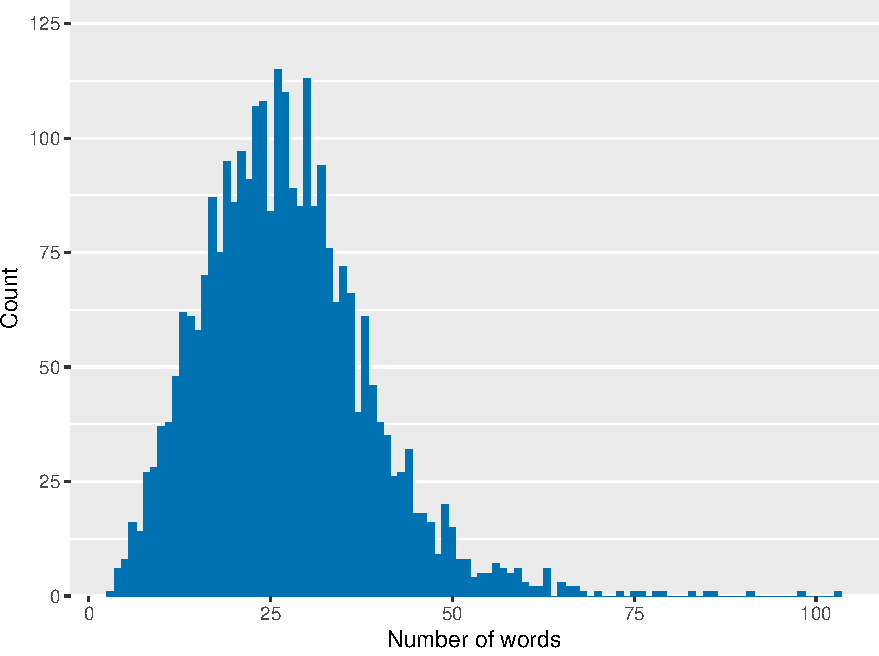
\includegraphics{thesis_files/figure-latex/sentenceLength-1} \hfill{}

\caption{Length of sentences}\label{fig:sentenceLength}
\end{figure}
The length is interesting, because it determines the chance that tokens
are observed more than once for each unit. In the newspaper sentences,
while some sentences are quite long, unique words very rarely appear
more than once; the mean number of times each word appears in each
sentence is 1.0187, meaning there is only a slim chance of observing a
given word more than once. This has implications for how the sentences
should be vectorized. Various strategies for vectorization are described
in the following chapter.

In addition to giving a description of the raw text as a whole, it is
also important to make sure that the text associated with each class
varies. This is important, because this variation will be used to train
the classifier to recognize text as belonging to each class. As shown
here, there seems to be some useful variation between the classes:
relevant sentences very often contain the word ``signed'' and
``agreed'', while these words are not present as often in the irrelevant
sentences.

This plot shows words word frequencies for each group of texts, as a
percentage of total words. Since, as mentioned above, the sentences were
selected as containing the words ``ceasefire'', ``truce'' and
``armistice'', these words are excluded from the plot. In addition, I
excluded stopwords from the plot. Stopwords are grammatical words like
prepositions and pronouns that occur very often in regular text (Bird
\emph{et al.} 2009: 60). The reason for excluding them here is that I am
interested in the differences in the more semantically loaded words,
like verbs and nouns. The exclusion of stopwords before classification
might also improve classifier performance, an assumption which is tested
in chapter 7. Note that both uppercase and lowercase words are shown;
these count as discrete tokens, unless the text is normalized by
lowercasing all words.
\begin{figure}

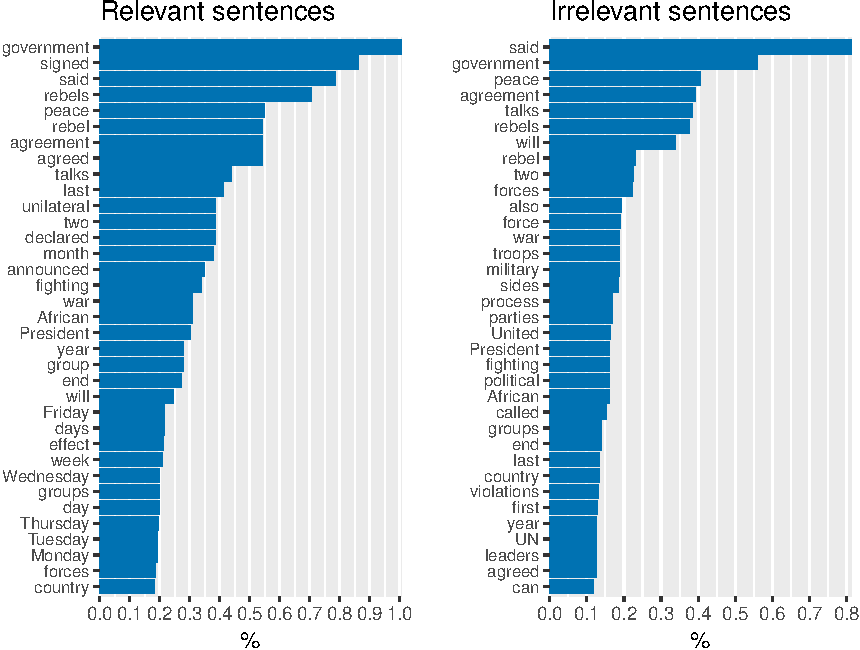
\includegraphics{thesis_files/figure-latex/wordFreq-1} \hfill{}

\caption{Word frequencies}\label{fig:wordFreq}
\end{figure}
\begin{table}[ht]
\centering
\begin{tabular}{rrr}
  \hline
 & Training & Holdout \\ 
  \hline
n & 2761.00 & 306.00 \\ 
  Relevant sentences & 870.00 & 109.00 \\ 
  Irrelevant sentences & 1891.00 & 197.00 \\ 
  Mean number of tokens & 26.02 & 26.55 \\ 
  Mean number of characters & 164.57 & 167.71 \\ 
  Unique tokens & 7367.00 & 2198.00 \\ 
   \hline
\end{tabular}
\caption{Data characteristics} 
\end{table}
\newpage

\chapter{Classification Methodology}\label{classification-methodology}

Several steps are necessary to use statistical learning techniques to
code outcomes similarly to human coders. The creation of structured data
depends on two steps; selecting a set of attributes with which cases are
represented, and classification based on these traits according to some
given classifier function.

As mentioned in the previous chapter, I used supervised learning to
estimate the classifier functions presented in the following chapter.
This means extrapolating the decision rules from a set of coded data and
applying these rules to new data. The estimation of the coding rule is
done through the application of statistical techniques, that mimic the
coding rule established in the training set.

In this chapter, I describe the technical methodology that was used to
estimate and evaluate classifiers in the following. I begin with a
brief, general overview of Machine Learning, defining key terms like
\emph{learning}, and drawing parallels to the previous discussion of
systematic observation.

Since there is no predefined ``best'' classifier algorithm for any given
problem, Thus, it is essential to test each algorithm using an
evaluation scheme. This methodology is used to select classifier
procedure that will be applied to a held-out partition of the labelled
data, to give a final evaluation of the effectiveness of statistical
learning methods in discerning between relevant and irrelevant
sentences.

I then describe the procedures that are used to classify text in the
following. Perhaps surprisingly, the classifier is not the focus
variable that is tested. I opted to use a simple variant, while instead
emphasizing different procedures related to the treatment and
representation of text.

Finally, I give a brief overview of the implementation of the different
steps. This description, along with links to the source code found in
the appendix, makes it possible to reliably and accurately reproduce the
work presented here, given a similar set of data.

\section{Machine Learning}\label{machine-learning}

Machine learning is a term used to describe computer systems that infer
functions from patterns in raw data. It can be considered a kind of
``artificial intelligence'' (Pustejovsky and Stubbs 2012: 37) in the
sense that it is able to ``learn'' its procedures from data, rather than
having to be explicitly instructed. An agent can be said to ``learn'' if
its performance is improved by way of observation (Russell and Norvig
2010: 693). A computer learns by way of statistical estimation,
computing models of relationships between traits and outcomes that have
been ``observed''.

Generally, learning, can be defined as the estimation of a procedure, or
function of observed cases based on the association of their attributes
and an outcome of interest. Thus, James \emph{et al.} (2013: 36)
describes statistical learning as an attempt to estimate a function
\(f\), where:
\begin{align}
y = f(x) + \epsilon \label{ml1}
\end{align}
This is done by observing cases expressed in terms of a vector of
features. Recall that I defined measurement as \(t = f(I)\)
(\ref{measurement}). In the definition of machine learning given above,
the attempt to estimate the function \(\hat{f}(x)\) behind measurements
\(y_1,y_2...y_i\) can thus be seen as an attempt to uncover \(f(I)\)~as
a function of the set \(I\) of attributes \(i_1,i_2...i_n\) of each unit
of observation \(u_1,u_2...u_i\).

There are two reasons for wanting to learn such a function from raw data
(James \emph{et al.} 2013: 17) : The first is to explore the
coefficients in the function to learn more about the relationship
between the variables, or rather, what has been learned about this
relationship. This is usually the purpose of traditional regression
analysis, where insight is gained from examining coefficients, that show
statistical correlations between different indicators with various
degrees of confidence.

The second reason is to use the learned function to predict new
outcomes. This is extremely useful when an outcome of interest is more
expensive or difficult to measure than the features (James \emph{et al.}
2013: 28). Consider this in the case of text classification; observing
manifest features of text is trivial, while measuring ``hidden''
information content, significance, or relevance is a much more difficult
task. In the present case, it is not possible to measure outright
whether a sentence is interesting or not to coders by, for example,
testing whether a certain symbol, letter or word is present. Statistical
learning, then, is used to create a procedure that infers the value of
this attribute, based on what is observable: The symbol content of each
sentence.

A basic dichotomy in machine learning is the distinction between
supervised learning and unsupervised learning (Grimmer and Stewart 2013:
2). The difference between these rather different approaches, is that
with supervised learning, the goal is to estimate a function of an
outcome variable that is observed, while with unsupervised learning, a
theorized number of outcomes are inferred from patterns in the data.

Supervised learning models are estimated using ``training data'', where
the outcome variable is given, while unsupervised models are used to
``discover'' an outcome variable as a pattern in the independent
variables. This process of ``teaching'' the model about the connection
between indicators and the outcome variable \(y\) means that
essentially, the outcome function \(f\) will be an imitation, or rather
extrapolation of the coding function that ``generated'' the outcomes in
the training data. This means that supervised learning and subsequent
classification must proceed from a set of data that has been labelled
(Grimmer and Stewart 2013: 3), as described in the previous chapter, and
that the validity of the outcomes of the function is dependent on the
validity of the labelling of the training data. The algorithm ``learns''
how to classify documents, mimicking the assumed decision rule \(f\)
applied by the human hand coders (Grimmer and Stewart 2013: 9).

It is clear from the definition given above that machine learning and
formal measurement are analogous processes. The basic premise is
estimating a function of a given set of traits, that will be used to
infer some unobserved trait of interest. Machine learning models can
thus be thought of as ``measuring instruments''.

Supervised models use the procedures and rules established in the
training data to establish the measuring procedure. This means that a
supervised learning model is a tool of \emph{extrapolation}. It is thus
very important to mindfully develop the rules with which the training
data is classified: Valid training data is a prerequisite for valid
outcomes using a trained model.

\section{Evaluation methodology}\label{evaluation-methodology}

There is no way to determine the ideal approach to estimating
\(\hat{y}\) a-priori. Measuring the performance of different approaches
is the only way of determining which procedures perform well in a given
context (Grimmer and Stewart 2013: 3). In addition to the classification
step, different strategies for expanding each unit into a corresponding
feature vector should also be considered.

Using flexible, powerful modelling techniques, it is possible to
estimate a function \(\hat{f}\) that will perfectly predict \(y\) for
each training case. This will inevitably result in an \emph{overfit}
model, however: A model that does not generalize well to new, unobserved
cases (James \emph{et al.} 2013: 22). The term \(\epsilon\)~in the
definition of statistical learning means that it must be assumed that
the training data contains some specific variance in addition to the
``common'' variance that we are trying to model (see
\ref{validityCoef}).

Fitting too flexible models to the data might lead to models that
express the specific variance of the training set, a situation called
``overfitting'' where the classifier is trained to recognize the
semantically trivial characteristics in the training data. These
characteristics are not useful for classifying the phenomenon of
interest more generally, but might be correlated with the phenomenon in
the training data.

Recall from chapter 4 that information relayed through language is
affected by the stochastic elements of language formulation; any given
piece of information could be expressed in multiple ways. What this
means is that each training case contains both uninteresting
idiosynchrasies and information; in the terms used to discuss validity,
we might say that each training case is affected by specific and general
variance.

To handle this problem, evaluation strategies should be designed so that
each procedure is tested on unseen data, that is not used to estimate
the procedure. This is done by splitting the data into separate
partitions, estimating the classifier using one partition, and applying
it to an ``unseen'' partition. In addition, a final ``holdout''
partition can be used to give a definitive score using data that has not
been used at all during preliminary evaluation of the development of the
model. Because the data used to calculate the metrics are not used in
estimating the model, the metrics give an indication of how well the
model will generalize, thus avoiding overly specific, overfit models.

Comparing \(y\) and \(\hat{y}\), the predicted and actual classification
of text in the unobserved data, it is possible to quantify model
performance directly by calculating several metrics that favor different
kinds of model performance. The choice of a performance metric affects
the choice of models, therefore it is important to reflect on the
characteristics of the different metrics.

\subsection{K-fold cross validation}\label{k-fold-cross-validation}

It is also important to consider different approaches to partitioning
the data. If data is scarce, the testing partition might be too small to
produce a useful metric. The partitioning of the data can be done in
several ways. For example, one might sample a percentage of the data
randomly, splitting it into two parts, training the model on one part,
and evaluating it on the other. The randomness ensures that the model is
representative of the whole data set.

However, if the data set is small, the respective partitions become to
small to yield reasonable results. Classifier procedures perform better
as the amount of training data increases. Training data is expensive to
produce, and will in almost every case be a scarce resource. Therefore,
it might be better to use a different strategy:

Resampling is a technique that involves estimating an equivalent model
from multiple randomly created partitions of the same data. With
multiple different random partitions, the resulting models will differ
slightly. Calculating evaluation metrics for each model gives a more
robust impression of how the modelling approach is performing.

One such approach is called K-fold cross validation (James \emph{et al.}
2013: 181). This involves splitting the data into \(K\) partitions,
called ``folds''. \(K\) models are then trained, excluding one part of
the data in each case, thus each model is trained on \(K-1\) folds.
Evaluating each model using the left-out fold gives a more robust and
complete picture of how the modelling strategy is working on the whole
of the data, as every data point is used for evaluation, yielding more
generalizable results.

In addition to the K-fold validation procedure, ten percent of the data
is ``held out'' from the process of specifying and testing the
procedures. This data is unseen until the final evaluation, and will
thus give a good indication of how well the classifiers generalize. This
is a good strategy, because the results from development testing data
might be biased towards good performance, since procedures are developed
and selected using only this data (Jurafsky and Martin 2018: 77).

\subsection{Metrics}\label{metrics}

When a classifier is used to predict scores for \(y\) where \(y\) is
already known, its performance can be evaluated in terms of how often it
classifies correctly. A Confusion Matrix (Fawcett 2006) is a way of
presenting the performance of a classifier, and can be used to calculate
additional performance measures.

In this matrix, the rows represent the hypothesized class of each case,
and the columns represent the true case. Given two possible values of
\(y\), P and N, four possible outcomes are possible: If the value of
\(y\) is P, the classifier can either produce a ``true'' P, TP, or a
``false'' N, FN. Conversely, if the value of \(y\)~is N, the classifier
can either produce a TN, or a FP:
\begin{table}[ht]
\centering
\begin{tabular}{rll}
  \hline
 & Actual N & Actual P \\ 
  \hline
Hypothesized N & TN & FN \\ 
  Hypothesized P & FP & TP \\ 
  Total & N & P \\ 
   \hline
\end{tabular}
\caption{Confusion matrix illustration} 
\end{table}
While the Confusion Matrix is a useful tool for evaluating classifiers
up front, when comparing classifier specifications, it is often useful
to express performance in terms of metrics, summarizing the matrix. From
the Confusion Matrix, it is possible to calculate several such metrics,
which summarize the performance of the classifier in various ways.
Choosing to focus on a particular performance metric is an important
decision when designing a classification scheme, as different metrics
emphasize different kinds of performance.

A natural point of departure is to calculate the ratio of \emph{correct
classifications} to \emph{total classifications}, called the
\emph{accuracy} of the procedure. The major diagonal of the confusion
matrix represents correct decisions, while the minor diagonal holds
erroneous decisions. From these, accuracy is defined as:
\begin{align*}
Accuracy &= \frac{TP + TN}{TP + FP + TN + FN}
\end{align*}
However, while accuracy is desirable in any case, an accurate classifier
is not necessarily useful. In a case where there are very few true
positive cases, a procedure yielding only negatives will achieve a very
high accuracy, while not being of much use in finding the positives
(Jurafsky and Martin 2018: 74).

From these, and the column totals \(N\) and \(P\), how many cases of
\(y=N\) and \(y=P\) there are in total, it is possible to calculate:
\begin{align*}
 Precision &= \frac{TP}{TP + FP}\\
 Recall &= \frac{TP}{P}
\end{align*}
Recall gives the ratio of \emph{correctly classified} cases P, to
\emph{actual} cases P, while precision gives the measure of
\emph{correctly classified} cases P to \emph{total classified} cases P.
Recall thus reflects the degree of coverage, while precision reflects
the credibility, or trustworthiness of predicted P.

In simpler terms, a more conservative classifier scores higher on
precision than recall (Fawcett 2006: 863). Importantly, high precision
and high recall tend to be mutually exclusive, (Chinchor and Diego 1992:
24). Thus, a choice must be made: If it is very important to catch all
the positive cases, and some noise in the outcome is acceptable, recall
should be prioritized. Conversely, if it is important that the cases
classified as positive are not actually negative, precision should be
prioritized (Hanna 2017: 13).

\subsubsection{F1 and ROC}\label{f1-and-roc}

A ``compromise'' between these two statistics is the F statistic. The F
statistic is calculated from precision and recall, and rewards models
with equal, strong precision and recall while punishing models with low
scores, or high but asymmetric scores in either statistic.
\begin{align*}
 F = \frac{(\beta^{2} + 1) \times Precision \times Recall}
          {\beta^{2}\times Precision + Recall}
\end{align*}
The balancing parameter \(\beta\) is used to determine the balance of
the effect of Precision and Recall. The special case where
\(\beta = 1\), making \(F\) equal to the harmonic mean of Precision and
Recall, is termed \(F1\). ``Weighting'' the F score towards either
Precision or Recall can be done based on considerations of the
importance of credibitlity versus coverage.

For the specific task of classifying sentences as either ``interesting''
or not for the coders, one must consider the importance of either
missing too many relevant sentences, or including too many irrelevant
sentences. While it may seem logical to avoid missing as many
potentially relevant sentences as possible, the system must also perform
well in filtering the information, as that is its main function in the
coding process. I therefore chose to weigh the measures equally, and to
rank the models according to their F1-score.

Lastly, I also present some approaches as points in ROC-space. ROC-space
is defined (Fawcett 2006: 862) as the two-dimensional space comprised of
the evaluation metric dimensions Recall and Fallout. Fallout is a
measurement of the number of cases with a true score of N, that have
been classified as P.
\begin{align*}
Fallout= FP / N
\end{align*}
When metrics calculated from a confusion matrix from a given procedure
are mapped to ROC space, the point indicates the degree of coverage,
Recall, versus what might be termed the ``trustworthiness'' of the
procedure, represented as Fallout. More lenient models will produce more
False Positives, but will also cover a larger array of the True
Positives. More conservative models, on the other hand, will discard
more True Positives as false, but will also produce fewer False
Positives, as illustrated here:
\begin{figure}

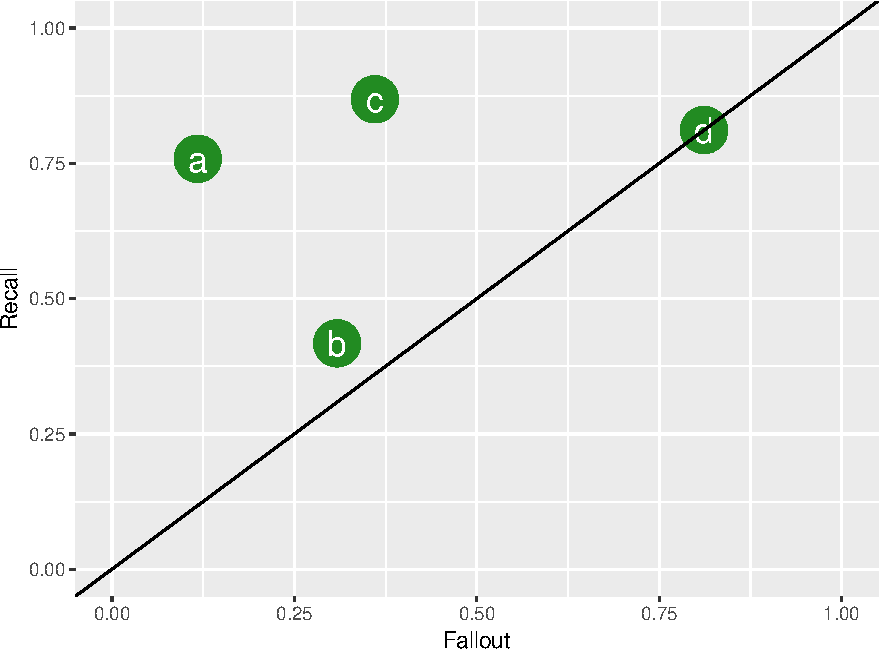
\includegraphics{thesis_files/figure-latex/rocToy-1} \hfill{}

\caption{Example ROC graph}\label{fig:rocToy}
\end{figure}
In this toy example, \(a\) is the model that combines a reasonable
Recall without encurring too much fallout. \(c\), on the other hand,
correctly classifies more positives, but also wrongly classifies many
negative cases as positives. Both \(b\) and \(d\) are dangerously close
to the line between 0,0 and 1,1; These models do not perform much better
than random guessing would.

The models \(a\) and \(c\) both perform well; choosing one of them
involves a substantial choice: Is it more important to catch as many
positives as possible, thus risking a less trustworthy set of
predictions? Or is the trustworthiness of the predictions the most
important element? This must be determined by considering the context in
which the results will be used.

\section{Procedure selection}\label{procedure-selection}

Classifications are produced by sending the text through a pipeline of
steps that might perform preliminary preprocessing, turns the raw text
into a vector representation, and classifies it using some sort of
classifier function. Any number of steps, algorithms and parameters
could be tested, but a selection is made to facilitate testing.

The reason for limiting the range of procedure variants that will be
considered is related to the exponential increase in variants that must
be evaluated; The number of procedures that must be tested increases
exponentially for each step that is considered. This makes it necessary
to select a subset of steps to focus on; I have chosen to consider
several preprocessing steps, instead of different classifiers.

Only two variants of the actual classification step will be considered
here; a Support Vector Machine (Cortes and Vapnik 1995) with and without
hyperparameter tuning. Support Vector Machines are a group of algoritms
that are commonly used for supervised machine learning (Pustejovsky and
Stubbs 2012: 39). SVM was chosen because it is considered one of the
best range of classifiers ``out of the box'' (James \emph{et al.} 2013:
337). The great advantage of SVM, along with the also common Logistic
Regression and Naïve Bayes models, is that it balances simplicity with
predictive power (Jurafsky and Martin 2018: 394), usually yielding
adequate results. In addition, SVM models do not requiring long training
cycles and complex tuning compared to more sophisticated approaches like
Neural Networks. It would of course be very interesting to apply more
advanced classification schemes to the task presented here, and compare
the results, but for the sake of parsimony, I have chosen to only
present results from using an SVM.

Support Vector Machine classifiers can be specified in several ways.
Again, limiting the range for the sake of parsimony, i only use a linear
kernel specification, which limits the range of hyperparameters to a
single parameter: C. C determines the amount of error that will be
tolerated by the separating hyperplane. Essentially, C determines the
``slackness'' of the separating rule; if C is small, the model is
tightly fit to the data, potentially increasing the risk of overfitting.
If C is large, on the other hand, the model might be underfit, and miss
the relevant relationship.

C is treated as a tuning parameter (James \emph{et al.} 2013: 347). This
means that determining an a-priori value for C is not possible; several
procedures must be estimated using cross-validation to determine which
C-value yields the best results on testing data. In the presentation in
the next chapter, the ``tuning'' step represents the inclusion of
C-tuning; otherwise, C is set to 1, the default value in the
implementation used here.

\subsection{Text as data}\label{text-as-data}

``Raw'' data like text, numbers and audio has no inherent vector
representation, and must be given one through the measurement of some
property or feature. This is called featurization. Featurization is
essentially just a given way of measuring one or several attributes of
an object to create an analyzable representation of it (Zheng and Casari
2018: 10).

Featurization is arguably the most important step when making a machine
learning system, and might have a very strong effect on classifier
performance (Bird \emph{et al.} 2009: 224). This resonates with how we
understand measurement, or indeed comprehension in general. What
attributes we choose to look at, or ignore, determines what we are able
to understand about some case. The procedures presented in the following
chapter largely differ in terms of the way text is vectorized.

Featurization means that each case is given a feature representation
\(x_1 ... x_i\). Any structured measurement procedure, computerized or
not, depends on some sort of ``featurization'', which is more or less
rigid. In the case of using computers, however, featurization must be
entirely schematic, and predefined. While, as I argued, all measurement
procedures can be more or less metaphorically viewed as mathematical
functions, computer classifiers are actual mathematical functions that
map vectors to outcomes. This means that all units must be given a
numeric vector representation, which expresses some set of features that
are determined to be relevant to the classification problem.

As briefly described in chapter 4, units of text such as sentences or
documents can be expressed in terms of a set of symbols. A
document-term-matrix (DTM) is a data set relation where documents are
represented through \emph{symbol occurrence}, with the word ``term''
used synonymously with ``symbol'' and ``token''. This means that the
variables are symbols, and the values are how often terms occur in each
document.
\begin{table}[ht]
\centering
\begin{tabular}{rllllll}
  \hline
 & Original & i & read & reading & text & that \\ 
  \hline
1 & I read text & 1 & 1 & 0 & 1 & 0 \\ 
  2 & Read that text & 0 & 1 & 0 & 1 & 1 \\ 
  3 & Text I read & 1 & 1 & 0 & 1 & 0 \\ 
  4 & Reading text & 0 & 0 & 1 & 1 & 0 \\ 
   \hline
\end{tabular}
\caption{Vectorization example} 
\end{table}
This is an example of a basic representation of text, the ``bag of
words'' approach. Under this representation, texts are transformed into
a dataset of count variables, expressing word occurrences. The values
can either be expressed in terms of either-or occurrences, that are
binary representations of whether a word occurs or not, or counts, that
are numerical values that express how many times a word appears.

In addition, the more sophisticated
Term-frequency-inverse-document-frequency transformation alters the
``weight'' of each word relative to their inverse document frequency, or
rather, how rare a word is in terms of how many documents it occurs in.
Common words are given less weight, while uncommon words are given more
weight.

There are several strategies that attempt to improve the baseline bag of
words approach. Each of these strategies aims to improve the performance
of subsequent classification, by either normalizing the values,
normalizing the data, or defining more complex features.

\subsubsection{Content and utility
words}\label{content-and-utility-words}

One such strategy involves selecting certain features that are assumed
to be more relevant than others. Only one set of such features is
considered for this approach: Stopwords. Stopwords are words that might
be expected to have little discriminatory power when classifying text.
These include prepositions, conjugations of ``to be'', and pronouns like
``them'' and ``he''.

The importance of including stopwords might be said to be related to the
required granularity of understanding necessary to discern between the
classes of text. In some cases, it might be necessary to discern between
texts using fine nuances in the way the author uses grammatical
``utility words'' like ``the'' and ``on'', but in other cases, these
words have no discriminatory value (Zheng and Casari 2018: 66). The list
of stopwords used in the current implementation is included in the
appendix.

Alternatively, instead of excluding stopwords, one might apply weights
to the coefficients of each word, relative to their Inverse Document
Frequency, or Term-Frequency-Inverse-Document-Frequency (Tfidf)
transformation attempts to reduce the weight of utility words, since
they appear in most documents, while retaining the weight of content
words, which are rarer (Jurafsky and Martin 2018: 508).

\subsubsection{Normalization}\label{normalization}

A second strategy involves normalization of symbols. The simplest
normalization is treating words that are capitalized and uncapitalized
as the same, by making all letters lowercase. If it is significantly
important whether words are capitalized, warranting this distinction,
lowercasing might be detrimental to performance, as it removes this
information. In many cases, however, it is not.

The normalization of numbers relates to how numbers are featurized:
Since each distinct number counts as a separate symbol, numbers increase
the number of features disproportionately to their assumed predictive
use. To handle this diversity, numbers can be transformed into a single
token, such as \texttt{*number*}. This retains the information that a
number is present, while collapsing the many distinct number-token
columns into a single column. The discriminatory power of having any
kind of number in a sentence is expectedly much greater than the
discriminatory power of observing specific numbers, at least in the
context of this classification problem.

Stemming is another kind of normalization that removes the distinction
between symbols in a courser way. Stemmers reduce each word to a root
stem, making distinct words with the same word stem appear the same.
This means that the words ``abstraction'', ``abstracting'',
``abstracted'' and ``abstract'' would all be stemmed and represented by
the symbol ``abstract''. While collapsing several such words into single
stems might significantly reduce the number of distinct symbols, and
thereby reduce the dimensionality of the data, it is also a heavy-handed
reduction of the information content of each text unit. The relevant
question when considering to include stemming is; is the discriminatory
value of suffixed words greater than stemmed words (Porter 1980). This
is, in any case, a difficult question to answer. Here, it is answered
empirically, by evaluating the effect of stemming on classifier
performance.

\subsubsection{N-gram featurization}\label{n-gram-featurization}

A third strategy involves the featurization step: A perhaps striking
fact about the bag-of-words representation of text is that it discards
information that is often vital for human text comprehension: The
sequence of symbols. Word sequence is an important syntactical component
in many languages, that determines the semantic meaning of text. The
tabular representation of texts in terms of symbol occurrence does not
retain this information.

Thus, using a basic bag-of-words approach rests upon the assumption that
the sequence of words is not useful for predicting \(y\). It is
worthwhile to evaluate this assumption, by including procedures that
vectorize the text in the form of n-grams. An n-gram is a representation
of n number of words in sequence. Two such n-gram representations are
considered here: Bigrams, and trigrams.

Since we are using statistical techniques to determine the significance
of each feature, why not include as many features as possible and let
the classifier sort them out? Again, this relates to the problem of
overfitting (Bird \emph{et al.} 2009: 225). If the classifier is allowed
to ``know too much'' about the training data, it might start modelling
idiosynchrasies rather than useful information. This makes the inclusion
of more information, such as by using n-grams, a trade-off.

\section{Implementation}\label{implementation}

In the following, all procedures were implemented using the software
library Scikit-Learn 0.19.1 (Pedregosa \emph{et al.} 2011). The SVM
procedures included with Scikit-Learn use Libsvm (Chih-Chung and
Chih-Jen 2011), a common implementation. In addition, some language
processing, including stemming and stopword-removal, is done using
Natural Language Toolkit 3.3 (Bird \emph{et al.} 2009). The framework
for building and testing classifiers was written in Python 3.6.5, and
most of the code for handling and presenting data was written in R
3.4.4. The source code used to train and evaluate the models, as well as
the source code used to render the thesis and produce the graphical
content in this thesis can be found by following links in the appendix.

\chapter{Results}\label{results}

In this chapter, I present the results of two batches of tests. The
first batch, where I test several algorithms on the training data using
K-fold cross validation is used to select the ``best'' algorithm. This
algorithm is then tested on the unseen held-out data, yielding a
generalizable result. The results from testing the text classifier were
positive. The best-performing specification achieved results that were
quite positive.

In addition to these numerical results, preliminary trials from the
data-making process at PRIO / ETH have also been quite positive. As an
integral part of the process of gathering data about ceasefires, the
classifier provides coders with an overview of the vast textual
material, providing relevance-ranked overviews of the many thousands of
sentences contained in the ``raw'' news material. Using these, coders
have reportedly been able to work quicker, both producing more data, and
auditing material that has already been gathered.

As part of the evaluation on the held-out data i also examine some
errors made by the system. These discussions might be fruitfully
considered when developing the system further, towards greater accuracy
and coverage. I also outline some of the many possible ways in which the
system can be improved by applying more sophisticated technologies.
These suggestions for further research, building on the findings
presented here, might lead to a more comprehensive automatic system for
creating useful conflict data.

\section{Procedure}\label{procedure}

Using the data described in chapter 5, several classifier algorithms
were created. The modelling step in each of these procedures is an
estimation of the ``manual'' procedure that was used to classify the
message units as either relevant or irrelevant, \(\hat{f}\), and is used
to extrapolate this procedure to produce predictions of relevance for
further coding work.

Determining what the ideal steps for processing and classifying the text
would be a-priori is not possible (Grimmer and Stewart 2013: 3), and so,
figuring out what steps to apply involves testing the performance of the
algorithms on coded data. 13 configuration are presented below. The
algorithm that performs best in the k-fold evaluation step is then used
to classify the held-out data, yielding a set of definitive metrics that
indicate how useful supervised learning might be for
relevance-classifying raw text in this specific problem domain.

What is a good score? This must, in any case, be defined in terms of the
task. There exists no general standard of passable scores for either of
the metrics presented here (Hanna 2017: 13). For this domain, however, I
would argue that the results attained by the best approach are quite
good, especially considering the relative simplicity of the classifier,
preprocessing and featurization schemes.

An even more advanced featurization, or classification step might have
yielded even better results, although the results clearly indicate that
the attempts to improve performance through slightly more sophisticated
procedures did not pay off in this case. The combination of parsimony
and performance makes the top-performing procedure a good alternative
for the task of ranking the relevance of sentences for coders, attaining
an F1 score of 0.78.

\section{Evaluation}\label{evaluation}
\begin{figure}

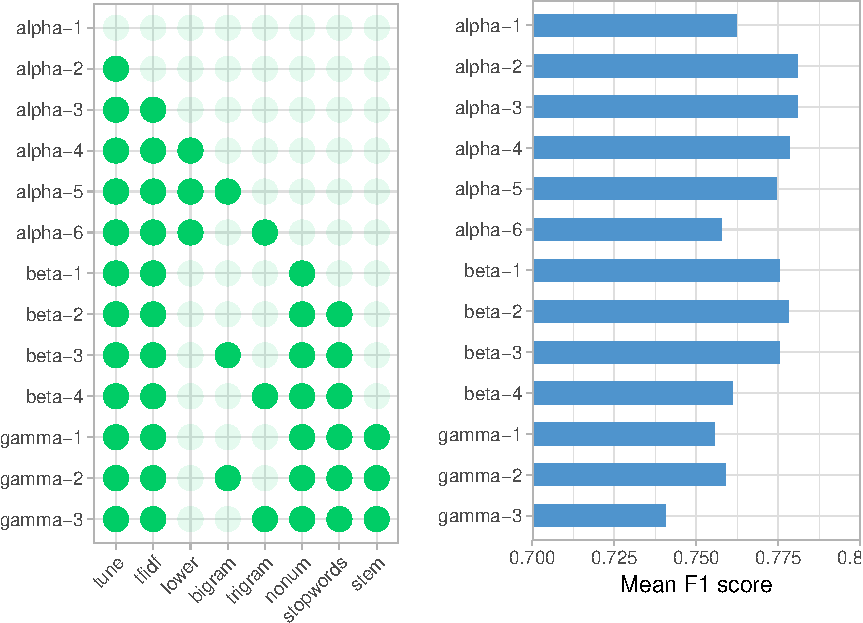
\includegraphics{thesis_files/figure-latex/modelsTable-1} \hfill{}

\caption{Procedure overview}\label{fig:modelsTable}
\end{figure}
13 different classifier configurations were evaluated. The number was,
in part, limited by practicality: The total number of combinations of 8
different steps is 256 . To facilitate the comparison, I chose to limit
the configurations into 3 ``families'' of models.

Each procedure was evaluated using 10 folds, meaning the procedure was
trained and tested ten separate times using different partitions for
training and testing. The scores are therefore quite robust. In the
table, the mean of these ten scores is show, for each procedure.

The Alpha family gradually introduces different steps, such as model
tuning, Tfidf-normalization lowercasing, and n-gram featurization. The
Beta family introduces number-word normalization and stopword removal,
using the best-performing combination from Alpha. Finally, Gamma
introduces stemming. Bigram and Trigram featurization is tested in all
three groups.

What is immediately apparent from this comparison, is that the different
approaches to modelling are quite similar in terms of performance. Note
that the scale on which the F1 parameter is displayed is heavily
compressed: The F1 parameter varies between 0 and 1, while F1 values
displayed here range between 0.74 and 0.78.

Still, there are certainly interesting differences in performance. Most
notably, the attempts to improve performance by including preprocessing
and n-gram featurization are actually detrimental to the F1 score. This
is not too surprising, considering the discussion of these steps in the
previous chapter: more advanced preprocessing and vectorization steps
might improve performance in some cases, but are not proven to be
effective in all cases: Their effectiveness rests on certain assumptions
about the text.

The best-performing model was selected from each of the model families,
and situated in ROC space. The points in this graph represent separate
scores, from each of the ten test folds. This plot shows that the
performance detriment in the gamma-family seems to stem from the fact
that the model yields slightly more false positives, while not gaining
any significant new amount of true positives. This is penalized by the
balancing parameter F1.
\begin{figure}

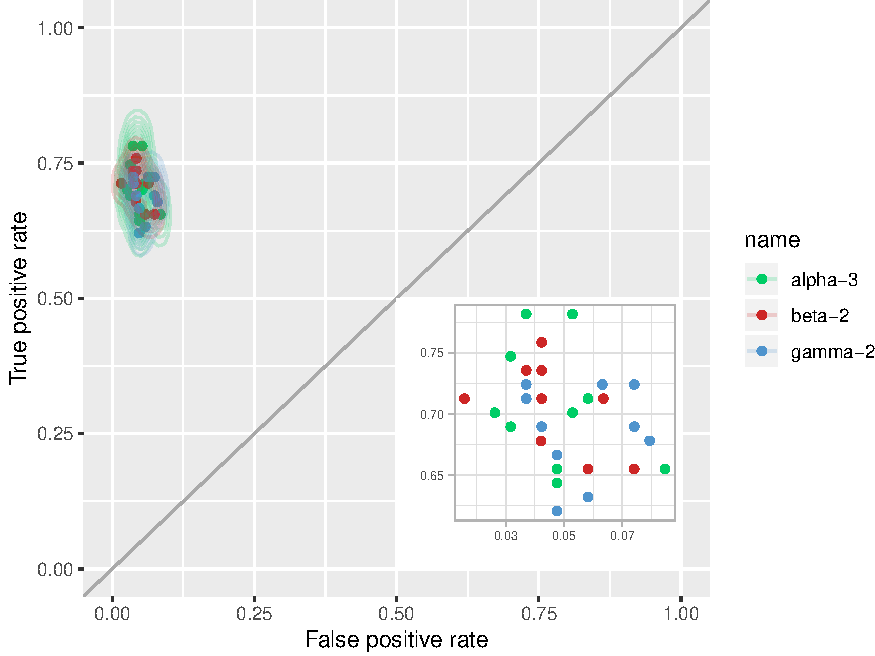
\includegraphics{thesis_files/figure-latex/rocPlot-1} \hfill{}

\caption{ROC procedure comparison}\label{fig:rocPlot}
\end{figure}
Again, it is quite clear that the models are not very different; in the
full extent of ROC-space it is difficult to tell them apart. While it
might be argued that the differences are so small that they are
attributable to random error, this conclusion would still favour the
best-performing procedure, alpha-3, since it is also the simplest
procedure, involving fewer steps than beta and gamma.

The top performing classifier, with a mean F1 score of 0.78, was
alpha-3.

alpha-3 thus seems to be the best \(\hat{f}\) for predicting \(y\) that
was attainable with the techniques attempted here, and the training data
that was used. It should, however, be noted that the difference between
the F1 value of the top performing classifier and the F1 value of the
worst performing one, gamma-3, is only 0.0404.

It is certainly interesting that the procedure that yielded the best
scores in the cross-validation evaluation was the simplest one. This is
not easily interpretable, but should be considered in light of the
discussion of these steps in the previous chapter. Feature selection
might be excluding certain features that are actually relevant, symbol
normalization like stemming and lowercasing might be removing important
nuances of information from the normalized symbols, and n-gram
vectorization seems to lead to an overproliferation of features, that
the model is not able to utilize effectively. Model tuning and
Term-frequency-inverse-document-frequency, however, yield slight
improvements over the baseline model.

\subsection{Holdout evaluation}\label{holdout-evaluation}

To evaluate the generalizability of alpha-3, the procedure was
subsequently tested on the held out data; data that has not been handled
during the development and testing of the procedures. The results
attained by attempting to classify the holdout data are more
generalizable, since the data has not been used to create the
classifier.

Since a majority of the cases in the holdout data are negative, meaning
that they are uninteresting to coders, it might be a useful reference
strategy to predict all the sentences as irrelevant, and calculate the
accuracy: This gives an accuracy of 64.38\%. Randomly guessing the class
in every case, with evenly balanced probabilities of 50/50 for each
class, gives an accuracy score of 0.53\%. Using alpha-3, on the other
hand, yields the following results:\newline
\begin{table}[ht]
\centering
\begin{tabular}{rrr}
  \hline
 & Negative & Positives \\ 
  \hline
Predicted N & 186 &  11 \\ 
  Predicted P &  28 &  81 \\ 
   \hline
\end{tabular}
\caption{Holdout confusion matrix} 
\end{table}
\newline
This translates to a precision score of 0.74 , a Recall score of 0.88 ,
an accuracy of 87.25\% , and an F1 score of 0.81. These scores seem to
indicate that the information about whether a sentence is relevant or
not for further coding yields itself quite well to classification; the
proposed lower boundary for acceptable F1 values for a similar
classification problem has been suggested as 0.65 (Hanna 2017: 13).

\subsection{Holdout error analysis}\label{holdout-error-analysis}

The errors made by alpha-3 might inform future work improvements to the
classifier. Browsing the sentences that were misclassified yields some
interesting reflections on how the classifier works. Along with the
coefficients estimated by the model, also called the feature weights, we
might better understand the errors made by the model. These are the ten
strongest coefficients in either direction:
\begin{flushleft}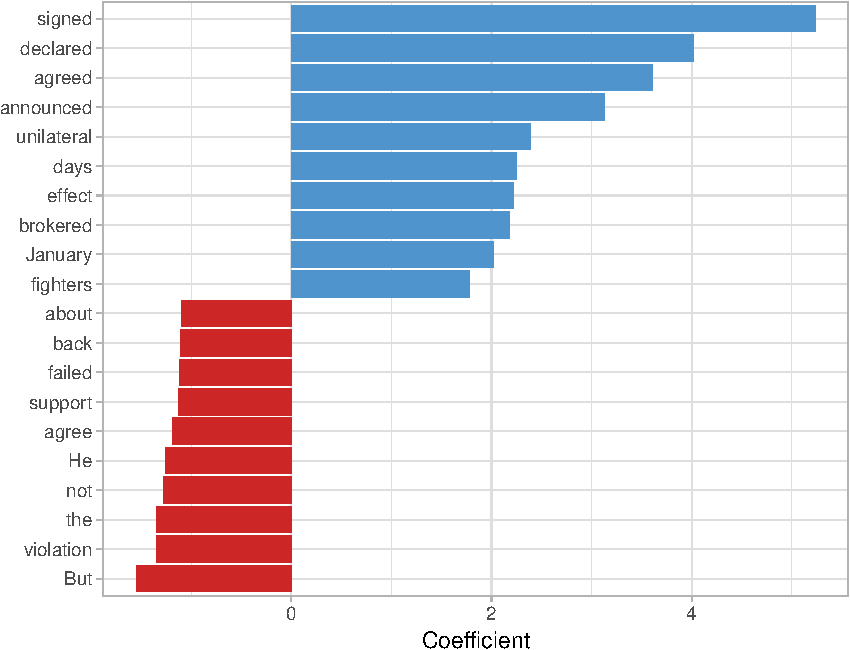
\includegraphics{thesis_files/figure-latex/wordCoefs-1} \end{flushleft}

\noindent
The four verbs that are most strongly correlated with a sentence being
interesting have much stronger coefficients than most other words,
particularly, and perhaps expectedly, the word ``signed''.

The verb ``to sign'', specifically the conjugated form ``signed'' which
corresponds to several conjugated forms of the verb, plays a significant
role in discerning between the sentences. Both of the ``false positive''
sentences contain the salient conjugation, that strongly correlate with
a sentence being interesting.

There were 28 false positive classifications. Two of these are:
\begin{itemize}
\tightlist
\item
  «A final and comprehensive ceasefire was to have been signed last
  month.»
\item
  «In the first place, there was no cease-fire agreement signed in
  Windhoek»
\end{itemize}
Parsing the sentences, however, we see that the semantic meaning of both
sentences does not, in fact, indicate that signing has taken place. The
fact that ``no cease-fire'' has been signed is a sufficiently complex
formulation to slip under the radar. Similarly, the complex verb
construction ``was to have been signed'', subtly negating the verb, is
not properly understood by the classifier. The passive-voice perfective
construction ``was to have been'' only appears once in the holdout data,
and does not appear in the training data.

Handling linguistic diversity is a matter of creating more training
data, as sufficient amounts of training data would contain cases where
the classifier is taught more advanced grammar than it is able to learn
from the present data.

Another interesting false positive sentence is:
\begin{itemize}
\tightlist
\item
  «A 1999 peace accord signed in Lusaka set a timetable for a ceasefire,
  the deployment of U.N. peacekeepers and a transition to democracy, but
  it has not been implemented.»
\end{itemize}
This sentence was strongly predicted to be true, but was manually
labelled as uninteresting. Figuring out how to handle this sort of
sentence, however, is harder, because it must involve some
disambiguation of the labelling rules: The sentence was labelled
uninteresting because it does not directly indicate the start of a
ceasefire, but an accord was signed. While it might be argued that this
sentence should in fact had been labelled as ``interesting'', since it
clearly indicates the signing of a peace accord, it might also be argued
that focus should remain on the start of actual events. In the last
case, the classifier can be made able to handle such ambiguous cases as
this one, given more training data.

There were 11 false negatives:
\begin{itemize}
\tightlist
\item
  «Although Kabila and the rebels have accused each other of violating
  the ceasefire deal that went into effect on September 1, there has
  been a substantial reduction in fighting.»
\end{itemize}
The negative, irrelevant sentences include a lot of mentions of
violations. Violation is strongly negatively correlated with a sentence
being interesting, and this is presumably true of other forms of the
stem ``violat'', like the above ``violating''. Despite mentions of
violations, the sentence also mentions in passing when a ceasefire went
into effect, rendering it interesting. This is overshadowed by the main
content of the text, however.
\begin{itemize}
\tightlist
\item
  For that reason, Israel's Security Cabinet unanimously rejected a U.S.
  proposal for a ceasefire on Friday, though Israel agreed to a 12-hour
  pause for Saturday.
\end{itemize}
This is a very difficult sentence to get right by simply using word
occurrence, since the rejection of a ceasefire proposal will almost
certainly render a sentence ``irrelevant'', while the sentence also
mentions a ``12-hour pause'', which was interpreted by the human coder
as indicating the start of a 12-hour ceasefire.
\begin{itemize}
\tightlist
\item
  The cease-fire is reportedly for one week.
\item
  They agree to a cease-fire.
\end{itemize}
These sentences were also, perhaps surprisingly, misclassified as
negative, while they are labelled as positive. This perhaps reflects the
detriment of using such short message units: Sentences of under ten
words contain very little information with which to discern between
positives and negatives. In addition to this, neither of these two
examples contain words that strongly indicate that they are positive. In
fact, the conjugation ``agree'' is quite negatively correlated with a
sentence being interesting, while the past-tense form ``agreed'' is
strongly positively correlated.

While some of these errors would have been very hard to avoid, owing to
grammatical complexity, and lack of information due to brevity, the
production of more training data would certainly help. In addition, it
might be interesting to experiment with alternative vectorization
strategies, such as Doc2Vec (Le and Mikolov 2014), that might facilitate
better handling of unorthodox wording.

\section{Further work}\label{further-work}

The classifier has already been ``put to work'' in the process of coding
the PRIO ceasefire-dataset. While it is still necessary to manually code
the details of each ceasefire, such as what the parties are, what
conflict the ceasefire pertains to, and the concrete dates on which it
begins and ends, the ``reccomendation system'' that has been implemented
with this classifier helps coders skim through the material much more
efficiently.

While no quantitative evaluation of the effect of the system on manual
coding performance has been conducted yet, anectodal information from
these first trials has been promising. Such an evaluation would require
considerable time and resources, involving multiple passes over the same
material to assess the effect of using the system, compared to not using
the system. It would, however, be very interesting to quantify the
alleged effect of using the reccommendations.

While these initial results have been promising, there are many
interesting ways in which the classifier could be improved: The accuracy
of the recommendations could be improved by adding more training data,
or using more sophisticated technologies. In addition, the system could
also be made to produce more information, in the form of partial coding,
mapping each sentence to a particular conflict, set of actors, or
similar contexts. This could lead to a more comprehensive
automatization, finally leading to a completely automatic system for
extracting interesting information from news data streams, such as has
been demonstrated by Hanna (2017), Osorio and Reyes (2017) and Schrodt
\emph{et al.} (1994) among others.

Adding more training data is the most obvious way to increase
performance of the relevance-rating step. Including data from more
conflicts and countries would improve the generalizability of the
classifier. Producing training data is laborious, but pays off in terms
of model performance; strategies for producing useful training data,
like using active learning (Rubens \emph{et al.} 2015: 809) might be
interesting to explore when creating more training data.

In addition, exploring the merit of more advanced vectorization and
classification techniques would be interesting. Vectorizing text using
sentence embeddings (Le and Mikolov 2014) would be particularly
interesting to explore. In addition, promising results have been
attained using Neural Networks (Beieler 2016) for the classification
step; a much more advanced and computationally intensive classifier
strategy.

Automating the coding process further would require the development of
more sophisticated algorithms for parsing and processing the sentences,
and extracting information. The system presented here is only a single
step towards a fully automated coder, but discerning between relevant
and irrelevant text units is an important first step in this process
(Hanna 2017: 7). Stepping up the ladder towards fully automated
information extraction, masses of unstructured information might be made
intelligible, and open to analysis. In addition, such a system could be
made to create the data in real-time, updating the data set
continuously.

There are many problems inherent in full automatization, including
include solving duplicate events (Schrodt and Van Brackle 2013: 30),
resolving ambiguous or difficult language constructions, and avoiding
semantically irrelevant material where wording might trick automated
systems. Sports reporting, where military metaphors are common, are a
typical challenge (Schrodt \emph{et al.} 2014: 4).

The approach demonstrated here, pairing human intelligence with machine
pre-filtering and recommendations is cost-effective and useful. Getting
the best of both words, human intelligence paired with machine
efficiency, the pairing manages to increase productivity while avoiding
the problems inherent in full automatization. It should also perhaps be
noted that the present system was developed in one year, by a single
undergraduate student, including the production of training data. This
means that development costs were negligible compared to the more
comprehensive coder projects mentioned above, developed by professional
scientists.

\chapter{Summary}\label{summary}

In this thesis, I have argued for, and demonstrated the automatization
of part of a data-creation process. Results seem to show that the system
is a useful addition to such a process, yielding generally useful
recommendations. The results show what kinds of procedures are most
effective, among a selection of simple preprocessing and classifier
configurations. The present system is a useful point of departure for
future information extraction, using either manual or automatic
techniques.

The work presented here proceeds from the idea that data is a necessary
prerequisite for the development of scientific theory. Facilitating more
efficent and precise data collection is an important part of expanding
the scope of testable hypotheses. This helps theory development, by both
enabling scrutiny of established theories, and perhaps also inspiring
new, more accurate ones.

The development of more accurate theory about how ceasefires interact
with conflict is the goal of the data collection program in which this
project is embedded. Refining our knowledge about ceasefires makes it
possible for policy-makers to design better interventions and mediation
strategies, potentially migitating and preventing more conflict.

Improving the efficiency and quality of data-production is a powerful
motivation, given the importance of achieving a better understanding of
conflict related phenomena, such as ceasefires.

Data collection is difficult and expensive. Thus, useful data is a
scarce commodity, requiring great investments of time and money to
develop. This problem is exacerbated when observational material is
ambiguous, requiring careful interpretation. Text is such an information
source, being a conduit of information that imparts stochastic variance
in the form of language idiosynchrasies, making the task of retreiving
useful information from large corpora of text very challenging. In
addition, in an age of information glut, ensuring the veracity of data
is important, and increasingly difficult.

The complexity of text as a medium of information makes it difficult to
develop data collection procedures. Using machine learning techniques,
decision functions are learned previously labelled training-data rather
than specified; this means that the careful interpretative wisdom humans
apply when retreiving information from text can be learned, and
subsequently applied by machines.

This is potentially a very effective way of approaching complex problems
such as text-labelling. With the formalization of data-collection, and
exposition of machine-learning theory, I hope to have shown that the
process of data-collection can be seen as analogous to the process of
estimating and applying machine-learning functions.

This was demonstrated and evaluated in the latter part of this thesis.
Building and evaluating several relatively simple approaches to machine
classifications, useful knowledge was gained about how to approach the
particular problem of relevance rating.

The findings presented here show that the application of machine
learning technology to the particular problem of discerning between
relevant and irrelevant material for coding ceasefires is very useful.
The primary issue of cost, which is prohibitive to data-collection, is
effectively mitigated by the application of automatic tools with
essentially no running cost. This also means that issues of data quality
can be handled more effectively, since more resources and focus can be
put into the development of sound procedures and algorithms rather than
the drudgework of manual data collection.

While the present system can be improved and extended in many
interesting ways, this proof of concept is a useful system in and of
itself, already having yielded useful results in the process of making a
dataset of ceasefires. The interdisciplinary approach, drawing on
computer science, statistical learning theory, formal scientific
methodology and conflict research which is demonstrated in this thesis
is a powerful approach. With the further development of social science
methodology leveraging the power and efficiency of computerized
inference, one might hope that enough empirical data can be produced to
enable researchers to gain comprehensive understanding of phenomena such
as ceasefires, thus perhaps allowing for the resolution of more
conflicts, preventing violence and devastation.

\newpage

\null

\chapter*{Appendix}\label{appendix}
\addcontentsline{toc}{chapter}{Appendix}

\section*{Distribution sentences and
ceasefires}\label{distribution-sentences-and-ceasefires}
\addcontentsline{toc}{section}{Distribution sentences and ceasefires}
\begin{table}[ht]
\centering
\begin{tabular}{rlrrr}
  \hline
 & Country & Ceasefires & Sentences & Sentences per Ceasefire \\ 
  \hline
1 & Burundi &  29 & 14949 & 515.48 \\ 
  2 & Central African Republic &  27 & 1390 & 51.48 \\ 
  3 & Colombia &  28 & 13729 & 490.32 \\ 
  4 & Djibouti &   5 & 670 & 134.00 \\ 
  5 & El Salvador &   3 & 2591 & 863.67 \\ 
  6 & Guatemala &   5 & 149 & 29.80 \\ 
  7 & Guinea-Bissau &   9 & 1249 & 138.78 \\ 
  8 & Ivory Coast &  11 & 12059 & 1096.27 \\ 
  9 & Kenya &  12 & 8458 & 704.83 \\ 
  10 & Lesotho &   1 & 263 & 263.00 \\ 
  11 & Liberia &  35 & 15038 & 429.66 \\ 
  12 & Mexico &  10 & 3045 & 304.50 \\ 
  13 & Morocco &   3 & 3983 & 1327.67 \\ 
  14 & Mozambique &  13 & 2799 & 215.31 \\ 
  15 & Nicaragua &  12 & 2163 & 180.25 \\ 
  16 & Niger &  11 & 1332 & 121.09 \\ 
  17 & Senegal &  10 & 594 & 59.40 \\ 
  18 & Sierra Leone &  15 & 9664 & 644.27 \\ 
  19 & Uganda &  24 & 17840 & 743.33 \\ 
   \hline
\end{tabular}
\end{table}\newpage
\section*{Coding of training
sentences}\label{coding-of-training-sentences}
\addcontentsline{toc}{section}{Coding of training sentences}

Basic criterion:
\begin{itemize}
\item Sentence contains any of the words "([Cc]ease-?fire|[Tt]ruce|[Aa]rmistice)" 
In the following, "ceasefire" is understood as either "ceasefire", "truce" or "armistice"
\end{itemize}
Sentences containing any of the following are interesting:
\begin{itemize}
\item ceasefire was declared
\item ceasefire was announced 
\item ceasefire was extended 
\item ceasefire went into effect 
\item *actor* is now observing ceasefire
\item A peace deal includes a ceasefire
\item ceasefire started/starts at *time*
\end{itemize}
Any of the following disqualify sentences as irrelevant:
\begin{itemize}
\item ceasefire provides for... (no time)
\item *actor* calls to respect ceasefire
\item *actor* calls for a ceasefire
\item *actor* offers a ceasefire
\item *actor* wants a ceasefire
\item References to an ongoing ceasefire 
\end{itemize}
\backmatter

\chapter*{References}\label{references}
\addcontentsline{toc}{chapter}{References}

\markboth{References}{References}

\noindent

\setlength{\parindent}{-0.20in} \setlength{\leftskip}{0.20in}
\setlength{\parskip}{8pt}

\hypertarget{refs}{}
\hypertarget{ref-adcock_measurement_2001}{}
Adcock, Robert and David Collier (2001) `Measurement validity: A shared
standard for qualitative and quantitative research', \emph{American
Political Science Review} 95(3): 529--546.

\hypertarget{ref-allen_introduction_1979}{}
Allen, Mary J. and Wendy M. Yen (1979) \emph{Introduction to measurement
theory}, Monterey, California: Brooks / Cole Publishing Co.

\hypertarget{ref-azar_ten_1975}{}
Azar, Edward E. (1975) `Ten issues in events research', in Edward E.
Azar and Joseph D. Ben-Dak, eds., \emph{Theory and practice of events
research}, 1--19, ch. I-1: Gordon; Breach Science Publishers.

\hypertarget{ref-beieler_generating_2016}{}
Beieler, John (2016) `Generating politically-relevant event data',
\emph{arXiv}.

\hypertarget{ref-bellamy_understanding_2010}{}
Bellamy, Alex J. and Paul D. Williams (2010) \emph{Understanding
peacekeeping}, Polity Press.

\hypertarget{ref-benoit_treating_2009}{}
Benoit, Kenneth, Michael Laver, and Slava Mikhaylov (2009) `Treating
words as data with error: Uncertainty in text statements of policy
positions', \emph{American Journal of Political Science} 53(2):
495--513.

\hypertarget{ref-bird_natural_2009}{}
Bird, Steven, Ewan Klein, and Edward Loper (2009) \emph{Natural language
processing with python}, O'reilly.

\hypertarget{ref-bratberg_tekstanalyse_2017}{}
Bratberg, Øyvind (2017) \emph{Tekstanalyse for samfunnsvitere}, Cappelen
Damm Akademisk.

\hypertarget{ref-bryder_innehallsanalys_1985}{}
Bryder, Tom (1985) \emph{Innehållsanalys som ide och metod}, Åbo
Akademis Kopieringssentral.

\hypertarget{ref-buhaug_geography_2002}{}
Buhaug, Halvard and Scott Gates (2002) `The geography of civil war',
39(4): 17.

\hypertarget{ref-chih-chung_libsvm_2011}{}
Chih-Chung, Chang and Lin Chih-Jen (2011) `LIBSVM - a library for
support vector machines', \emph{ACM Transactions on Intelligent Systems
and Technology} 2(3): 1--27.

\hypertarget{ref-chinchor_muc-4_1992}{}
Chinchor, Nancy and San Diego (1992) `MUC-4 EVALUATION METRICS', 8,
McLean, Virginia.

\hypertarget{ref-chojnacki_event_2012}{}
Chojnacki, Sven, Christian Ickler, Michael Spies, and John Wiesel (2012)
`Event data on armed conflict and security: New perspectives, old
challenges, and some solutions', \emph{International Interactions}
38(4): 382--401.

\hypertarget{ref-cioffi-revilla_introduction_2017}{}
Cioffi-Revilla, Claudio (2017) \emph{Introduction to computational
social science}, New York, NY: Springer Berlin Heidelberg.

\hypertarget{ref-codd_relational_1970}{}
Codd, E.F. (1970) `A relational model of data for large shared data
banks', 13(6): 11.

\hypertarget{ref-cortes_support-vector_1995}{}
Cortes, Corinna and Vladimir Vapnik (1995) `Support-vector networks',
\emph{Machine Learning} 20(3): 273--297.

\hypertarget{ref-date_database_2001}{}
Date, C. J. (2001) \emph{The database relational model}, Addison-Wesley
Publishing Company.

\hypertarget{ref-douglass_measuring_2018}{}
Douglass, Rex W. and Kristen A. Harkness (2018) `Measuring the landscape
of civil war: Evaluating geographic coding decisions with historic data
from the mau mau rebellion', \emph{Journal of Peace Research} 55(2):
190--205.

\hypertarget{ref-dulic_peace_2011}{}
Dulic, Tomislav (2011) `Peace research and source criticism', in
Christine Hoglund and Magnus Oberg, eds., \emph{Understanding peace
research}, 35--47, Routledge.

\hypertarget{ref-dumas_losses_1923}{}
Dumas, Samuel and K. O. Vedel-Pedersen (1923) \emph{Losses of life
caused by war}, Oxford, United Kingdom: Clarendon Press.

\hypertarget{ref-fawcett_introduction_2006}{}
Fawcett, Tom (2006) `An introduction to ROC analysis', \emph{Pattern
Recognition Letters} 27(8): 861--874.

\hypertarget{ref-fearon_rationalist_1995}{}
Fearon, James D. (1995) `Rationalist explanations for war',
\emph{International Organization} 49(3): 37.

\hypertarget{ref-fortna_scraps_2003}{}
Fortna, Virginia Page (2003) `Scraps of paper? Agreements and the
durability of peace', \emph{International Organization} 57(2).

\hypertarget{ref-gerring_case_2008}{}
Gerring, John (2008) \emph{Case study research}, Cambridge University
Press.

\hypertarget{ref-gleditsch_data_2014}{}
Gleditsch, Kristian Skrede, Nils W. Metternich, and Andrea Ruggeri
(2014) `Data and progress in peace and conflict research', \emph{Journal
of Peace Research} 51(2): 301--314.

\hypertarget{ref-gleditsch_armed_2002}{}
Gleditsch, Nils Petter, Peter Wallensteen, Mikael Eriksson, Margareta
Sollenberg, and Håvard Strand (2002) `Armed conflict 1946-2001: A new
dataset', \emph{Journal of Peace Research} 39(5): 615--637.

\hypertarget{ref-grimmer_text_2013}{}
Grimmer, Justin and Brandon M. Stewart (2013) `Text as data: The promise
and pitfalls of automatic content analysis methods for political texts',
\emph{Political Analysis} 21(3): 267--297.

\hypertarget{ref-hanna_mpeds_2017}{}
Hanna, Alex (2017) `MPEDS automating the generation of protest event
data', \emph{SocArXiv}: 40.

\hypertarget{ref-holsti_content_1969}{}
Holsti, Ole R. (1969) \emph{Content analysis for the social sciences and
humanities}, Philippines: Addison-Wesley Publishing Company.

\hypertarget{ref-huang_big_2018}{}
Huang, Jingwei (2018) `From big data to knowledge: Issues of provenance,
trust, and scientific computing integrity', in \emph{2018 IEEE
international conference on big data (big data)}, 2197--2205, Seattle,
WA, USA: IEEE.

\hypertarget{ref-hunt_experiments_1966}{}
Hunt, Earl B., Janet Marin, and Phillip J. Stone (1966)
\emph{Experiments in induction}, Academic Press.

\hypertarget{ref-james_introduction_2013}{}
James, Gareth, Daniela Witten, Trevor Hastie, and Robert Tibshirani,
eds. (2013) \emph{An introduction to statistical learning: With
applications in r}, New York: Springer.

\hypertarget{ref-jurafsky_speech_2018}{}
Jurafsky, Daniel and James H. Martin (2018) \emph{Speech and language
processing}, Third (draft).

\hypertarget{ref-kerlinger_foundations_1973}{}
Kerlinger, Fred N. (1973) \emph{Foundations of behavioural research},
2nd ed. Holt, Rinehart; Winston.

\hypertarget{ref-king_designing_1994}{}
King, Gary, Robert O. Keohane, and Sidney Verba (1994) \emph{Designing
social inquiry}, Princeton University Press.

\hypertarget{ref-kreutz_how_2010}{}
Kreutz, Joakim (2010) `How and when armed conflicts end: Introducing the
UCDP conflict termination dataset', \emph{Journal of Peace Research}
47(2): 243--250.

\hypertarget{ref-krippendorff_content_2004}{}
Krippendorff, Klaus (2004) \emph{Content analysis: An introduction to
its methodology}, SAGE Publications.

\hypertarget{ref-le_distributed_2014}{}
Le, Quoc V. and Tomas Mikolov (2014) `Distributed representations of
sentences and documents', \emph{arXiv:1405.4053 {[}cs{]}}.

\hypertarget{ref-leng_toward_1977}{}
Leng, Russell J. and J. David Singer (1977) `Toward a multi-theoretical
typology of international behaviour', in Mario Bunge, Johan Galtung, and
Malitza Mircea, eds., \emph{Mathematical approaches to international
relations}, 71--94, 1, Romanian Academy of Social; Political Sciences.

\hypertarget{ref-mahieu_when_2007}{}
Mahieu, Sylvie (2007) `When should mediators interrupt a civil war? The
best timing for a ceasefire', \emph{International Negotiation} 12(2):
207--228.

\hypertarget{ref-mason_when_2011}{}
Mason, David T., Mehmet Gurses, Patrick T. Brandt, and Jason Michael
Quinn (2011) `When civil wars recur: Conditions for durable peace after
civil wars: When civil wars recur', \emph{International Studies
Perspectives} 12(2): 171--189.

\hypertarget{ref-mcclelland_acute_1961}{}
McClelland, Charles A. (1961) `The acute international crisis',
\emph{World Politics} 14(1): 182--204.

\hypertarget{ref-milton-edwards_warriors_2017}{}
Milton-Edwards, Beverley (2017) `The warriors break: Hamas and the
limits of ceasefire beyond tactical pause', \emph{International
Peacekeeping} 24(2): 212--235.

\hypertarget{ref-morgenthau_politics_1948}{}
Morgenthau, Hans J. (1948) \emph{Politics among nations}, 7th ed. McGraw
Hill.

\hypertarget{ref-neuendorf_content_2017}{}
Neuendorf, Kimberly A. (2017) \emph{The content analysis guidebook}, 2nd
ed. SAGE.

\hypertarget{ref-oberg_gathering_2011}{}
Oberg, Magnus and Margareta Sollenberg (2011) `Gathering conflict
information using news sources', in Christine Hoglund and Magnus Oberg,
eds., \emph{Understanding peace research}, 47--73, Routledge.

\hypertarget{ref-osorio_supervised_2017}{}
Osorio, Javier and Alejandro Reyes (2017) `Supervised event coding from
text written in spanish: Introducing eventus ID', \emph{Social Science
Computer Review} 35(3): 406--416.

\hypertarget{ref-pedregosa_scikit-learn:_2011}{}
Pedregosa, Fabian \emph{et al.} (2011) `Scikit-learn: Machine learning
in python', \emph{Journal of Machine Learning Research} 12: 2825--2830.

\hypertarget{ref-porter_algorithm_1980}{}
Porter, Martin (1980) `An algorithm for suffix stripping',
\emph{Program} 14(3): 130--137.

\hypertarget{ref-pustejovsky_natural_2012}{}
Pustejovsky, James and Amber Stubbs (2012) \emph{Natural language
annotation for machine learning}, O'reilly.

\hypertarget{ref-raleigh_geographies_2015}{}
Raleigh, Clionadh (2015) `Geographies of conflict', in John Agnew,
Virginie Mamadouh, Anna J. Secor, and Joanne Sharp, eds., \emph{The
wiley blackwell companion to political geography}, 86--99, Chichester,
UK: John Wiley \& Sons, Ltd.

\hypertarget{ref-richardson_statistics_1960}{}
Richardson, Lewis Fry (1960) \emph{Statistics of deadly quarrels},
Chicago: Boxwood Press.

\hypertarget{ref-rubens_active_2015}{}
Rubens, Neil, Mehdi Elahi, and Masashi Sugiyama (2015) `Active learning
in recommender systems', in Francesco Ricci, Lior Rokach, and Bracha
Shapira, eds., \emph{Recommender systems handbook}, 809--846, New York,
NY: Springer Science+Business Media.

\hypertarget{ref-russell_artificial_2010}{}
Russell, Stuart and Peter Norvig (2010) \emph{Artificial intelligence: A
modern approach}, 3rd ed. Prentice Hall.

\hypertarget{ref-russett_note_1977}{}
Russett, Bruce (1977) `A note on techniques for controlling data error',
in Mario Bunge, Johan Galtung, and Malitza Mircea, eds.,
\emph{Mathematical approaches to international relations}, 94--109, 1,
Romanian Academy of Social; Political Sciences.

\hypertarget{ref-salehyan_best_2015}{}
Salehyan, Idean (2015) `Best practices in the collection of conflict
data', \emph{Journal of Peace Research} 52(1): 105--109.

\hypertarget{ref-schoon_why_2018}{}
Schoon, Eric W. (2018) `Why does armed conflict begin again? A new
analytic approach', \emph{International Journal of Comparative
Sociology}: 36.

\hypertarget{ref-schrodt_automated_2013}{}
Schrodt, Philip A. and David Van Brackle (2013) `Automated coding of
political event data', in V.S. Subrahmanian, ed., \emph{Handbook of
computational approaches to counterterrorism}, 23--49, New York, NY:
Springer New York.

\hypertarget{ref-schrodt_threes_2014}{}
Schrodt, Philip A., John Beieler, and Muhammed Idris (2014) `Three's a
charm?: Open event data coding with EL:DIABLO, PETRARCH, and the open
event data alliance.', 24, Toronto.

\hypertarget{ref-schrodt_keds:_1994}{}
Schrodt, Philip A., Shannon G. Davis, and Judith L. Weddle (1994) `KEDS:
A program for the machine coding of event data', \emph{Social Science
Computer Review} 12(4): 561--587.

\hypertarget{ref-simmhan_survey_2005}{}
Simmhan, Yogesh L., Beth Plale, and Dennis Gannon (2005) `A survey of
data provenance in e-science', \emph{ACM SIGMOD Record} 34(3): 31.

\hypertarget{ref-singer_data-making_1965}{}
Singer, J. David (1965) `Data-making in international relations',
\emph{Behavioural Science} 10(1): 68--80.

\hypertarget{ref-singer_variables_1982}{}
Singer, J. David (1982) `Variables, indicators and data: The measurement
problem in macropolitical research', \emph{Social Science History} 6(2):
181--217.

\hypertarget{ref-singer_wages_1972}{}
Singer, J. David and Melvin Small (1972) \emph{The wages of war
1816-1965: A statistical handbook}, John Wiley \& Sons.

\hypertarget{ref-stevens_theory_1946}{}
Stevens, S. S. (1946) `On the theory of scales of measurement',
\emph{Science, New Series} 103(2684): 677--680.

\hypertarget{ref-stone_general_1966}{}
Stone, Phillip J., Dexter C. Dunphy, Marshall S. Smith, and Daniel M.
Ogilvie (1966) \emph{The general enquirer: A computer approach to
content analysis}, MIT Press.

\hypertarget{ref-sundberg_systematic_2011}{}
Sundberg, Ralph and Lotta Harbom (2011) `Systematic data collection', in
Christine Hoglund and Magnus Oberg, eds., \emph{Understanding peace
research}, 91--114, Routledge.

\hypertarget{ref-wallensteen_understanding_2012}{}
Wallensteen, Peter (2012) \emph{Understanding conflict resolution}, 3rd
ed. SAGE.

\hypertarget{ref-wickham_tidy_2014}{}
Wickham, Hadley (2014) `Tidy data', \emph{Journal of Statistical
Software} 59(10): 1--23.

\hypertarget{ref-woolley_using_2000}{}
Woolley, John T. (2000) `Using media-based data in studies of politics',
\emph{American Journal of Political Science} 44(1): 156.

\hypertarget{ref-wueest_using_2013}{}
Wueest, Bruno, Klaus Rothenhäusler, and Swen Hutter (2013) `Using
computational linguistics to enhance protest event analysis', \emph{SSRN
Electronic Journal}.

\hypertarget{ref-zheng_feature_2018}{}
Zheng, Alice and Amanda Casari (2018) \emph{Feature engineering for
machine learning}, O'reilly.


% Index?

\end{document}
